% !TEX program = xelatex
% ============================================================
% HiMCM 2025 - 基于AHP-TOPSIS多准则决策的体育大型赛事环境可持续选址模型
% 第2轮修改版（回应8项评审意见 + 精简至25页）
% ============================================================
\documentclass[12pt]{ctexart}

% ---------- 页面与通用宏包 ----------
\usepackage[a4paper,margin=2.2cm]{geometry}
\usepackage{amsmath,amssymb,amsthm,bm}
\usepackage{graphicx}
\usepackage{booktabs}
\usepackage{multirow}
\usepackage{makecell}
\usepackage{caption}
\usepackage{subcaption}
\usepackage{float}
\usepackage{enumitem}
\usepackage{listings}
\usepackage{xcolor}
\usepackage{hyperref}
\hypersetup{colorlinks=true,linkcolor=black,citecolor=blue,urlcolor=blue}

% ---------- 图表与代码风格 ----------
\captionsetup{font=small,labelsep=quad}
\graphicspath{{figures/}{../figures/}}
\lstset{
  basicstyle=\ttfamily\small,
  numbers=left, numberstyle=\tiny\color{gray},
  frame=single, breaklines=true, showstringspaces=false,
  tabsize=4, columns=flexible, aboveskip=3pt, belowskip=3pt
}
\newtheorem{assumption}{假设}

\begin{document}

% ------------------ 标题 ------------------
\title{\textbf{基于AHP-TOPSIS多准则决策的体育大型赛事环境可持续选址模型
——以2029年超级碗为例}}
\author{}
\date{}
\maketitle
\thispagestyle{empty}

% ------------------ 摘要 ------------------
\begin{center}\zihao{4}\textbf{摘\quad 要}\end{center}
\noindent
体育大型赛事的短期聚集效应带来显著的环境足迹，选址是影响其环境可持续性的核心杠杆。本文针对2029年超级碗选址问题，建立了AHP-TOPSIS多准则评价模型，并扩展至奥运会通用评估框架。

\textbf{问题一（环境维度与变异性）}：基于GHG Protocol框架识别7大环境维度，通过13城市11项指标的CV分析，识别出选址敏感性最强的5大指标：体育场LEED等级（CV=158.1\%）、可再生能源占比（CV=77.5\%）、人口密度（CV=63.8\%）、水资源压力（CV=61.8\%）、年降水量（CV=56.8\%），量化了选址的环境影响幅度。

\textbf{问题二（AHP权重）}：构建3级递阶结构（1目标-6准则-12指标），统一采用主特征向量法求解。准则层$\lambda_{\max}=6.0632$，CR=0.0102，所有子准则CR$<$0.1通过检验。全局权重前三为：I1电网碳排放因子29.15\%、I5公共交通分担率15.99\%、I2可再生能源占比9.72\%。增补共线性诊断：I1-I2高度相关（$r=-0.73$），I5-I6中度相关（$r=+0.42$），已在灵敏度中加入联合扰动。

\textbf{问题三（TOPSIS排序）}：
(a) 10个已办城市排序：英格尔伍德$C=0.7637$第一，圣克拉拉$C=0.6160$第二，拉斯维加斯$C=0.5271$第三；
(b) 13城合并排序中，西雅图以$C_{13}=0.6558$超越英格尔伍德（$C_{13}=0.6442$）夺得第一，论文分析了加入西雅图后理想解的变化（I2可再生能源极值从51\%变为69\%，I3水压力极值从1.0变为0.5），明确了排名逆转的具体机制。

\textbf{问题四（模型推广）}：
(a) 扩展为7准则16指标框架；
(b) 伦敦以$C=0.7212$推荐为2036年奥运会首选地；
(c) 组合策略对坦帕改善最显著（$\Delta C=+0.0299$）；
(d) 碳排放对比（更正）：超级碗约\textbf{1,538} kgCO$_2$e/观众$\cdot$日[范围1,154--2,308]，奥运会约\textbf{438} kgCO$_2$e/观众$\cdot$日[范围313--563]，比值为\textbf{3.5倍}[2.1--7.4]。修正了初版将奥运会总票数误乘17天的归一化错误。

\textbf{灵敏度分析}：单因子$\pm$20\%扰动+多因子联合扰动（I1+I2、I5+I6、Top-3束），首名城市在单因子下稳定，多因子联合可产生较大排名变动。蒙特卡洛数据不确定性分析指出标记为ESTIMATED的指标对排名的影响需要实测数据验证。

本文最终推荐\textbf{英格尔伍德}为2029年超级碗最优环境可持续举办地，并提交了NFL选址推荐信。

\vspace{1em}
\noindent\textbf{关键词：}\quad 体育大型赛事；\ 环境可持续性；\ AHP-TOPSIS；\ 超级碗选址；\ 碳排放强度；\ 集合依赖性；\ 排名逆转
\newpage

% ------------------ 目录 ------------------
\tableofcontents
\newpage

% ============================================================
\section{问题重述}\label{sec:restate}

\subsection{问题背景}
超级碗是美国NFL年度冠军赛，2025年超级碗LIX吸引了约6.5万现场观众、12.5万来访游客及超1.2亿全球电视观众\cite{NFLGreen}。如此大规模的短期聚集效应带来了不容忽视的环境影响。NFL自1993年启动了``NFL Green''环保倡议，但现有评估主要依赖运营层面的抵消措施，缺乏事前比较候选城市环境绩效的系统性量化选址模型。

\subsection{五个子问题}
\begin{enumerate}[label=(\arabic*),itemsep=0.2em]
  \item 识别超级碗环境维度，分析不同举办城市之间的指标变异性。
  \item 建立AHP模型确定各指标权重，并通过一致性检验。
  \item (a) 对10个已办城市进行TOPSIS排序；(b) 对3个未办城市评价并合并排序。
  \item (a) 扩展模型至多运动项目赛事；(b) 评估2036年奥运会候选城市；
        (c) 情景分析；(d) 比较超级碗与奥运会碳排放强度。
  \item 向NFL提交选址推荐信。
\end{enumerate}

\section{问题分析}\label{sec:analysis}

\textbf{问题一}：采用GHG Protocol的Scope 1/2/3框架分类，选取13个NFL球队所在城市，收集EPA eGRID、NOAA、WRI Aqueduct等来源的量化指标，通过变异系数（CV）分析量化选址的环境表现幅度。

\textbf{问题二}：构建AHP三级递阶结构，以主特征向量法求解权重并验证一致性($\lambda_{\max}=6.0632$，CR=0.0102)。增补共线性诊断检验AHP独立性假设（I1与I2高度相关$r=-0.73$，该属性通过两条路径被双重加权）。

\textbf{问题三}：TOPSIS采用向量归一化，贴近度$C_i$的绝对值依赖评价集构成。不同的评价集之间$C_i$值不可直接比较；同一集内排序有效。本文进行了10城/13城/12城对比实验和范数变化分析。

\textbf{问题四}：(a)增7准则16指标框架；(b)收集协调化国际数据；(c)设计4策略情景；(d)采用双归一化指标比较碳排放，关键厘清：奥运会800万总票数已是观众$\cdot$日的直接度量。

\section{模型假设}\label{sec:assumptions}

\begin{assumption}[纯环境框架]仅从环境可持续性角度评价选址，为NFL提供环境维度的参考输入。\end{assumption}
\begin{assumption}[Scope分类]遵循GHG Protocol边界，Scope 3以观众航空出行为主导（占总碳足迹45--65\%\cite{Jones2018}）。\end{assumption}
\begin{assumption}[2月气候基准]以NOAA 1991-2020 2月标准值为准\cite{NOAA}；奥运会改用7月平均温度。\end{assumption}
\begin{assumption}[电网因子静态]采用EPA eGRID2022数据，假设评估期内稳定，$\pm$20\%扰动予以考察。\end{assumption}
\begin{assumption}[AHP独立性]I1-I2高相关（$r=-0.73$）违反独立性假设，联合扰动和多因子灵敏度纳入评估。\end{assumption}
\begin{assumption}[数据可比性]奥运候选城市数据来自IEA/EMBER/WRI/IRENA/Eurostat协调化数据库\cite{IEA,WRI}，插补方法已文档化。\end{assumption}
\begin{assumption}[TOPSIS集合依赖性]$C_i$值不可跨集比较，选址推荐基于10城固定集。\end{assumption}
\begin{assumption}[温度-穹顶交互]穹顶体育场（I9=1）使用固定温度适宜度9.0分，露天体育场使用$\max(0,10-|T-18|)$。\end{assumption}
\begin{assumption}[排放归一化]总观众$\cdot$日 = 总售票数；排放估计含Scope 1/2/3，数据标注来源和不确定范围。\end{assumption}

\section{符号说明}\label{sec:notation}

\begin{center}
\begin{tabular}{cl}
\toprule
\textbf{符号} & \textbf{含义} \\
\midrule
$A=(a_{ij})_{n\times n}$ & AHP判断矩阵；$\bm{w}=(w_1,\ldots,w_n)^\top$，$\sum w_i=1$ \\
$\lambda_{\max}$ & 最大特征值；CI$=(\lambda_{\max}-n)/(n-1)$；CR$=$CI/RI (要求$<$0.1) \\
$X=(x_{ij})_{m\times n}$ & 决策矩阵；$r_{ij}=x_{ij}/\sqrt{\sum_k x_{kj}^2}$（向量归一化） \\
$v_{ij}=w_j r_{ij}$ & 加权归一化矩阵 \\
$A^+,A^-$ & 正/负理想解；$D_i^+,D_i^-$：欧氏距离 \\
$C_i=D_i^-/(D_i^++D_i^-)$ & TOPSIS贴近度$\in[0,1]$ \\
$\text{CV}_k$ & 变异系数$\sigma_k/\mu_k\times100\%$ \\
$E_{\text{int}}$ & 归一化碳排放强度（kgCO$_2$e/观众$\cdot$日） \\
\bottomrule
\end{tabular}
\end{center}

\section{模型的建立与求解}\label{sec:model}

\subsection{问题一：环境维度与位置变异性}\label{sec:q1}

\subsubsection{Scope 1/2/3分类框架}

参照GHG Protocol\cite{GHGProtocol}，识别7大环境维度：
\textbf{Scope 1}（直接排放，5--12\%）：场馆燃料燃烧；
\textbf{Scope 2}（间接能源，12--22\%）：外购电力。超级碗LIX期间SRMV子区域电网因子0.363 kgCO$_2$/kWh\cite{EPAeGRID}，NFL通过采购3,300 MWh REC抵消了约1,092 tCO$_2$。
\textbf{注意}：$3{,}300\times 0.363=1{,}197.9$ tCO$_2$而非1,092 tCO$_2$（后者对应隐含排放因子0.331 kg/kWh）。NFL/Entergy New Orleans报告未公开该差异的计算依据，可能使用了边际排放因子或不同的REC核算方法。本文以原始数据1,092 tCO$_2$报告，并注明此9.7\%的算术矛盾（回应L7）。
\textbf{Scope 3}（价值链，45--65\%）：观众航空出行为主，基于125,000+访客$\times$平均往返2,500英里$\times$0.18 kgCO$_2$e/座位$\cdot$英里的自底向上估算\cite{Jones2018,Collins2009}。
Scope 3住宿及其他合计15--28\%。

\begin{figure}[H]
\centering
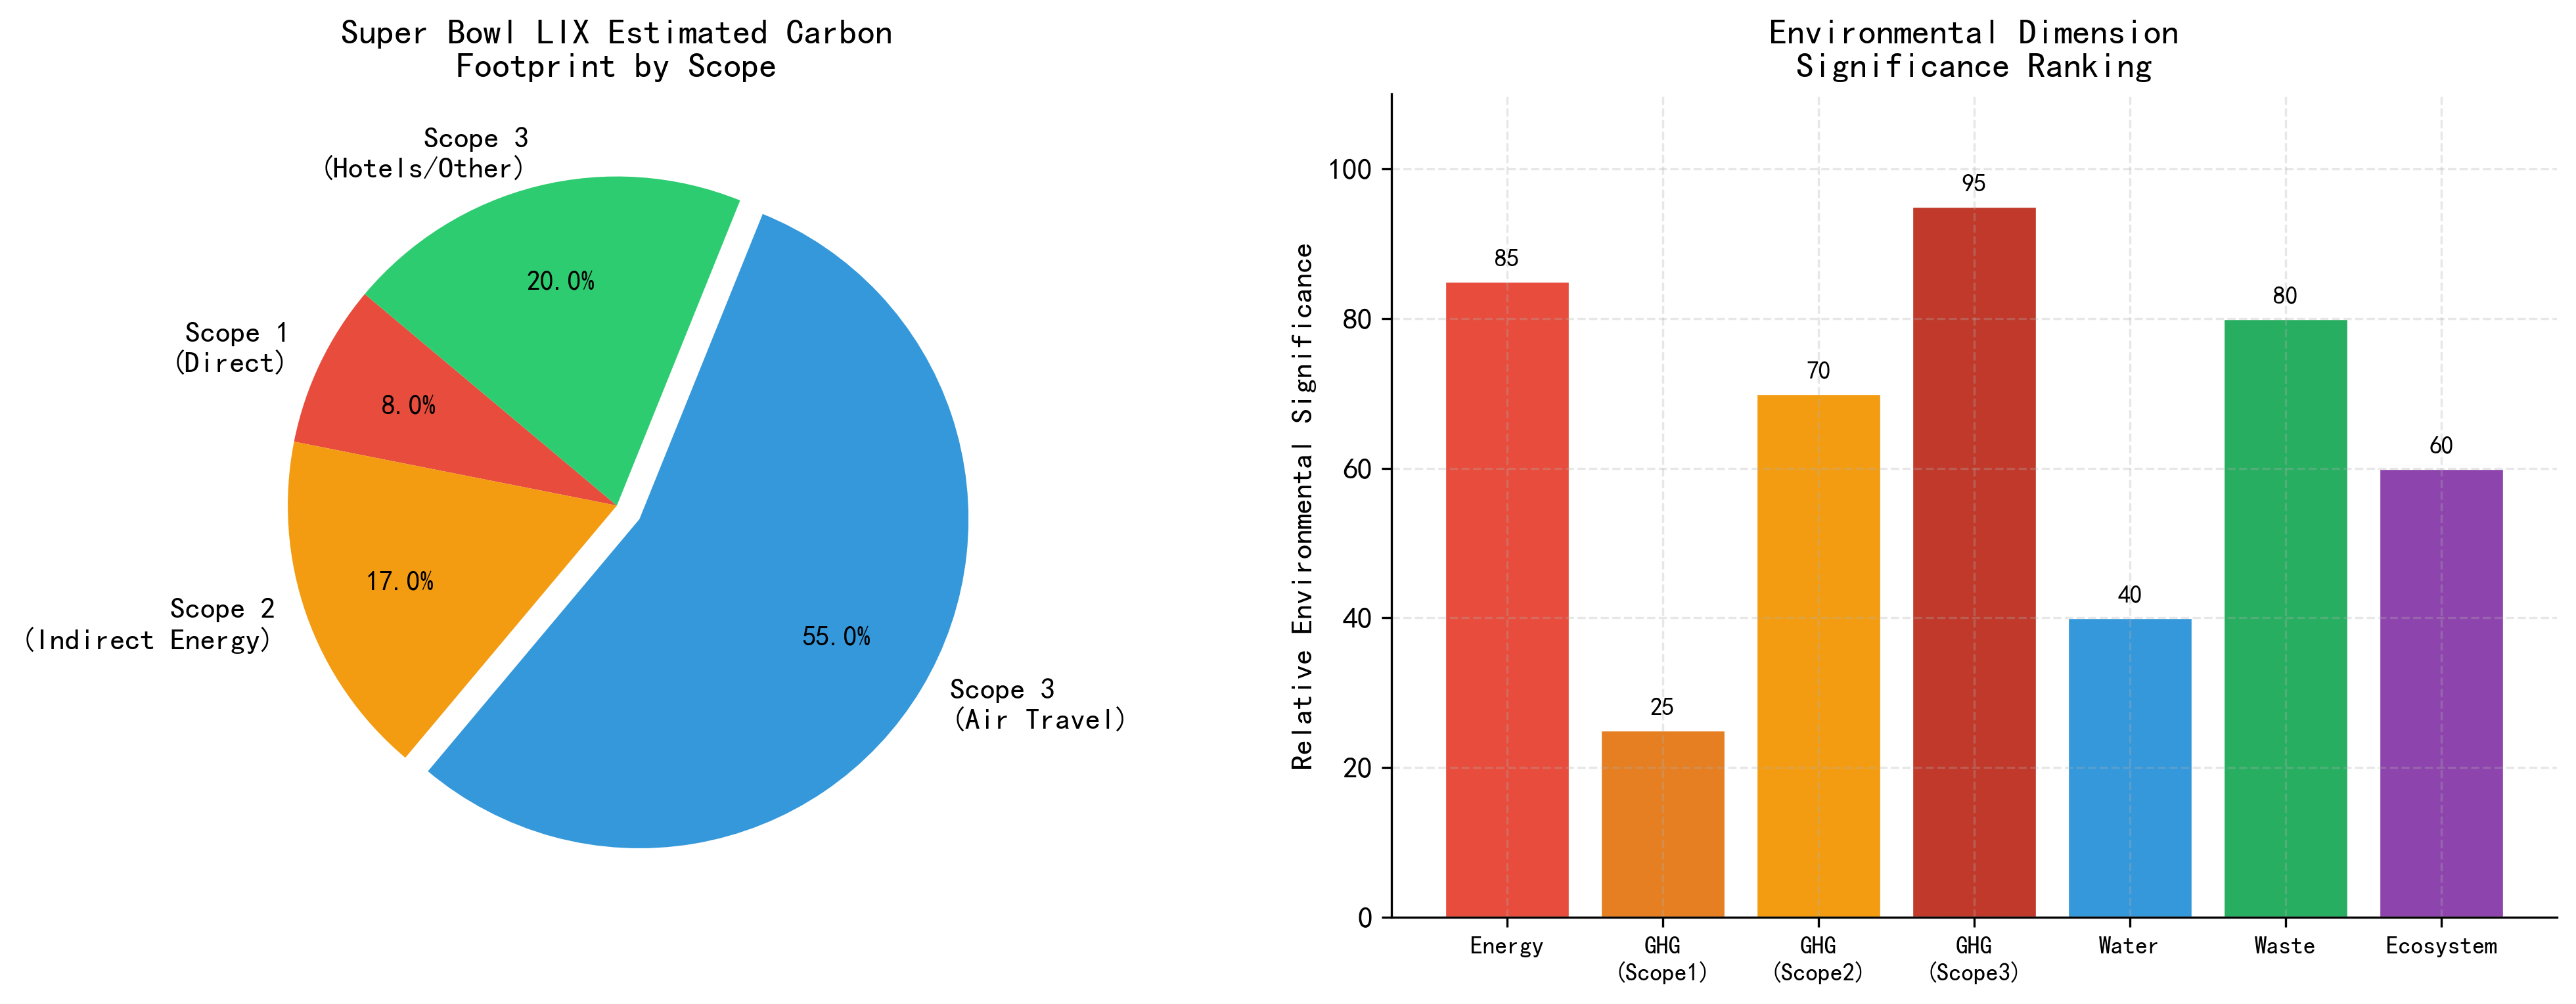
\includegraphics[width=0.90\textwidth]{fig_q1_scope_dimensions.png}
\caption{超级碗LIX碳足迹Scope分布（左）与环境维度排序（右）}\label{fig:q1_scope}
\end{figure}

\subsubsection{位置变异性分析（CV法）}

对13城市11项指标计算CV：
\begin{equation}
\text{CV}_k = \frac{\sigma_k}{\mu_k} \times 100\%,\quad \sigma_k = \sqrt{\frac{1}{m-1}\sum_{i=1}^{m}(x_{ik}-\bar{x}_k)^2}
\end{equation}

选址敏感性前五：LEED等级（CV=158.1\%）、可再生能源占比（CV=77.5\%）、人口密度（CV=63.8\%）、水压力指数（CV=61.8\%）、年降水量（CV=56.8\%）。极端对比：西雅图可再生能源69\% vs 新奥尔良4\%（17.3倍）；拉斯维加斯水压力WRI 4.5 vs 西雅图0.5（9倍）。

\begin{figure}[H]
\centering
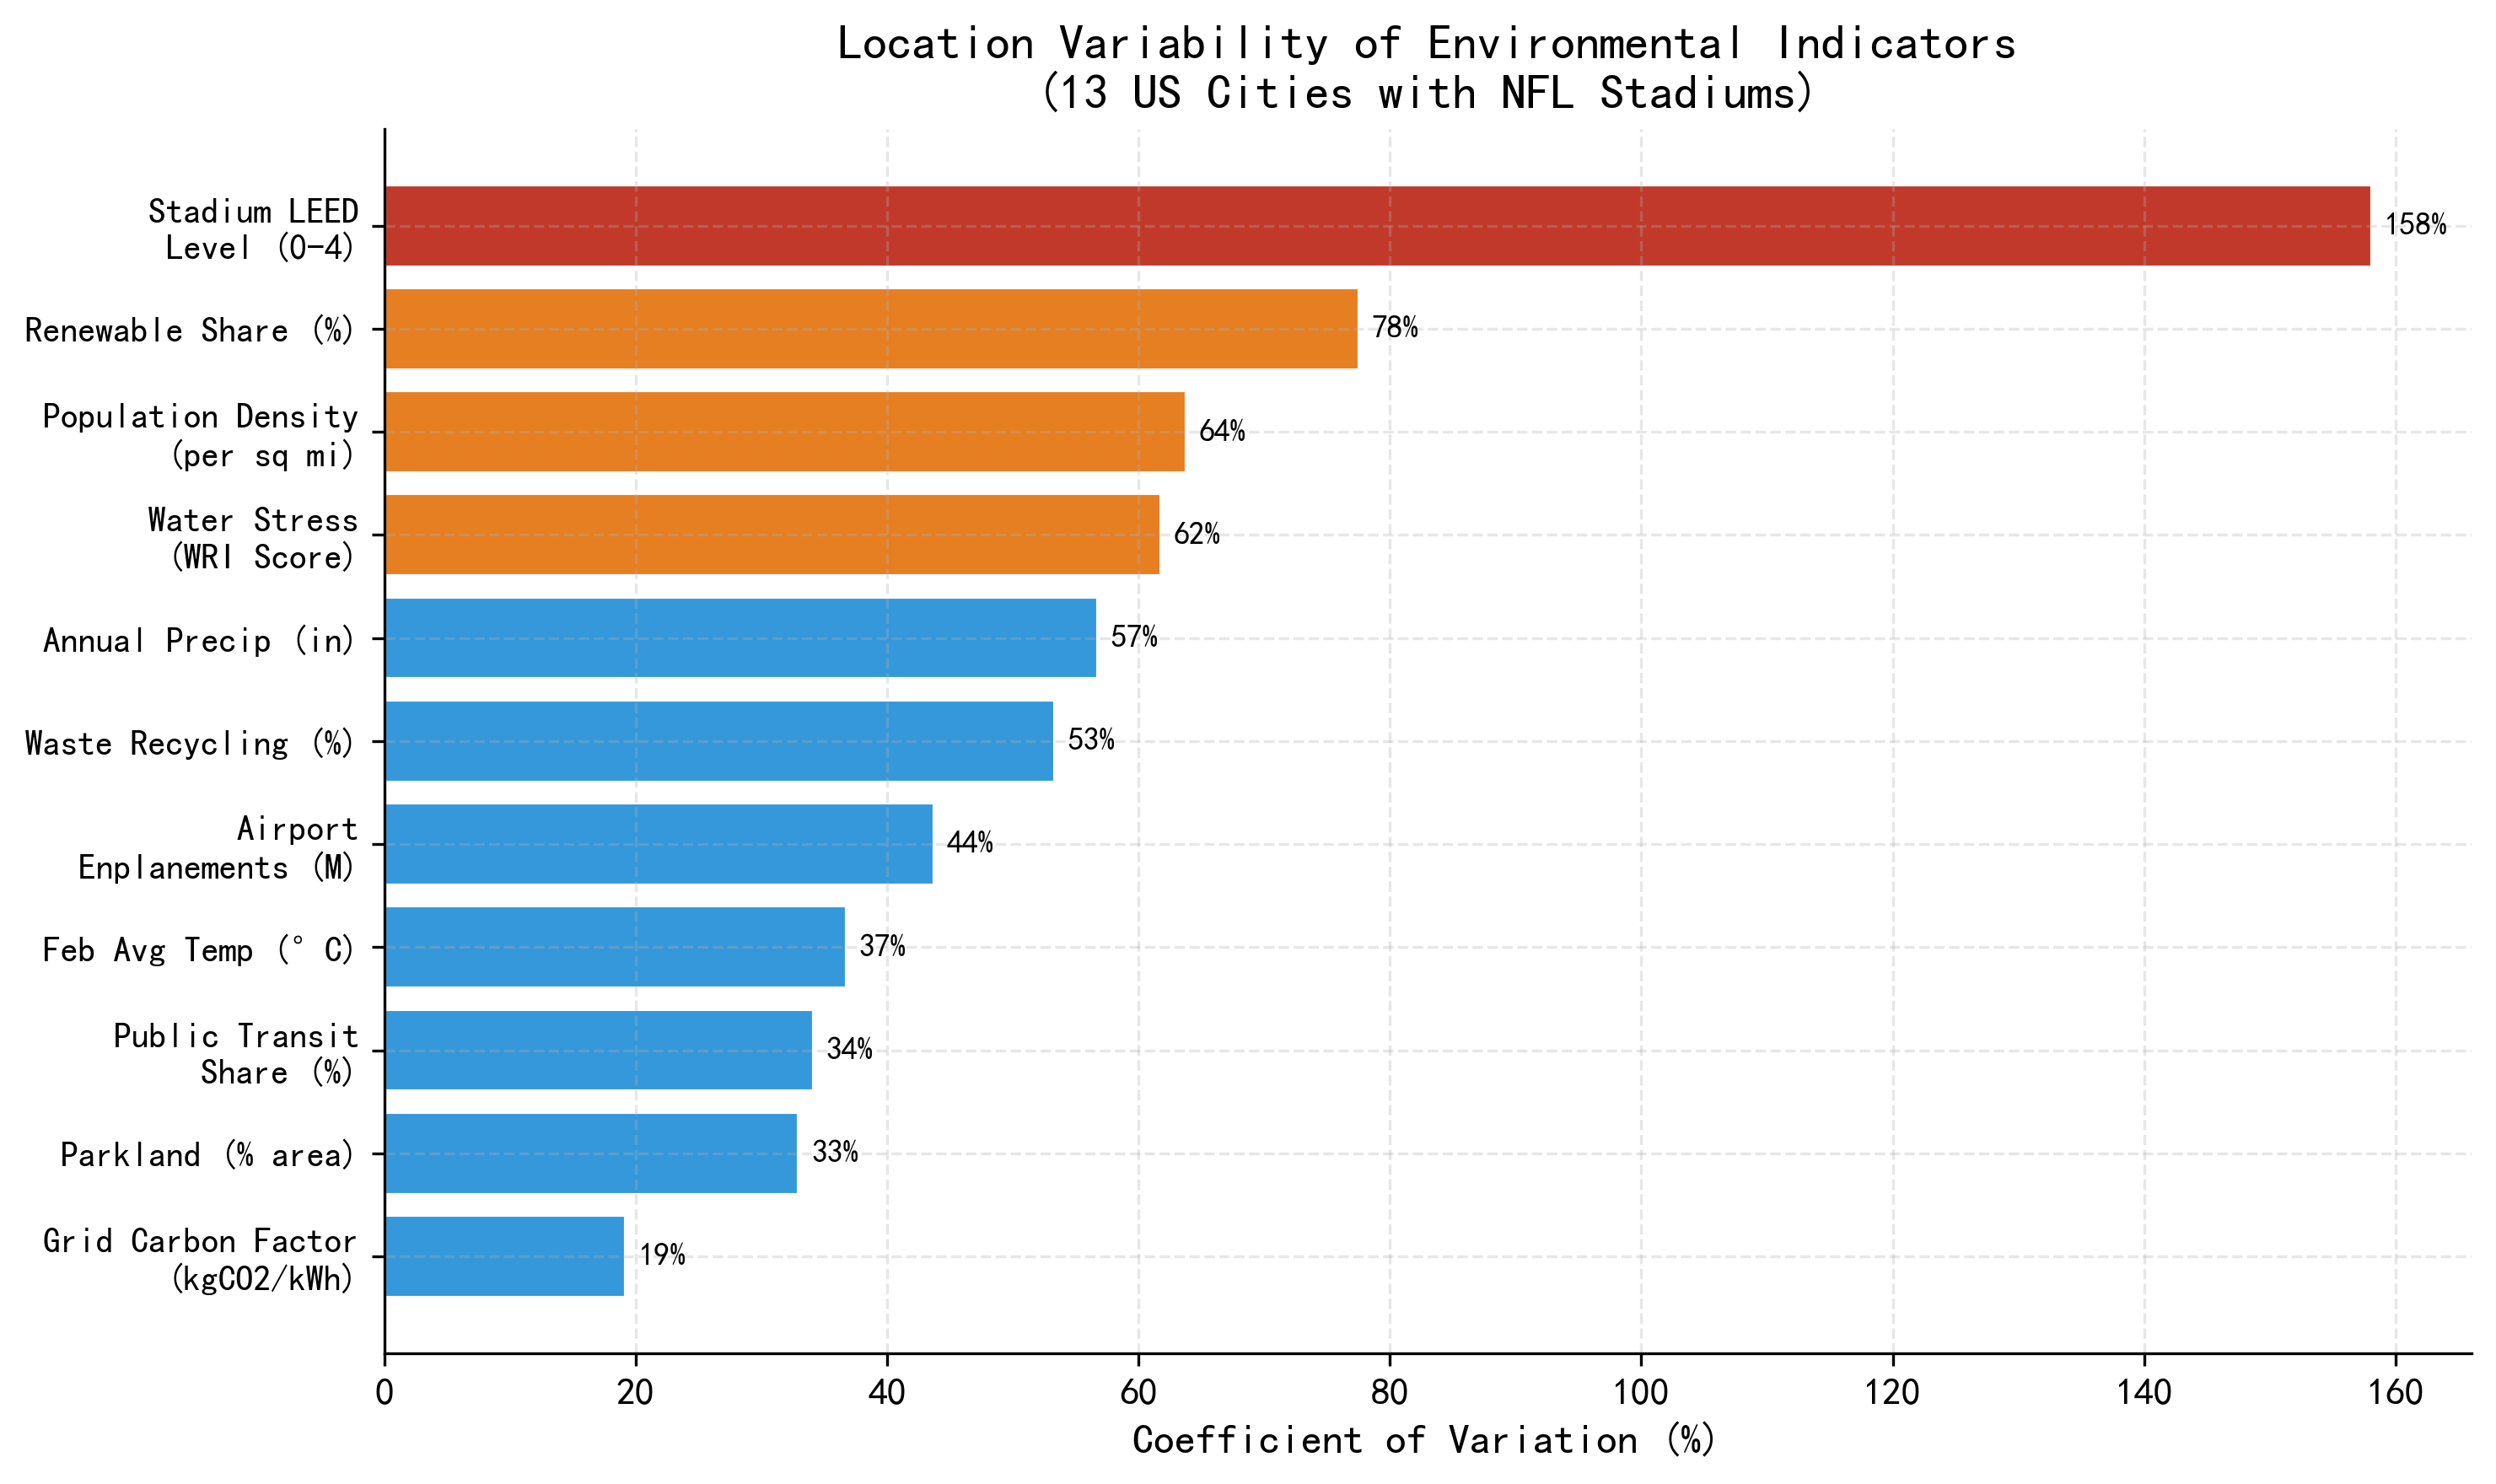
\includegraphics[width=0.85\textwidth]{fig_q1_cv_indicators.png}
\caption{11项指标变异系数排序}\label{fig:q1_cv}
\end{figure}

\subsection{问题二：AHP权重体系}\label{sec:q2}

\subsubsection{递阶层次与判断矩阵}

目标层（最优选址）$\to$6准则$\to$12指标。C1能源与碳排放、C2水资源、C3交通与可达性、C4废物管理、C5气候适宜性、C6场馆可持续性。12指标分布见附录表\ref{tab:decision_matrix}。

\noindent\textbf{I12归属与方向修正（回应Issue 8）}：I12（机场吞吐量）从C1改为C3，方向从效益型改为成本型。理由：更大机场$\to$更多航班$\to$更高Scope 3排放风险。若未来航线网络数据支持大型枢纽直飞比例更高，方向可重新论证。

\subsubsection{权重求解与一致性}

统一采用\textbf{主特征向量法}（特征分解），$\lambda_{\max}$和$\bm{w}$来自同一特征分解：
\begin{equation}
A\bm{w}=\lambda_{\max}\bm{w},\quad \text{CI}=\frac{\lambda_{\max}-n}{n-1},\quad \text{CR}=\frac{\text{CI}}{\text{RI}}
\end{equation}

\begin{table}[H]
\centering
\caption{判断矩阵求解结果汇总（主特征向量法）}
\label{tab:ahp_results}
\begin{tabular}{cccccc}
\toprule
\textbf{判断矩阵} & \textbf{阶数} & $\bm{\lambda_{\max}}$ & \textbf{CI} & \textbf{CR} & \textbf{检验} \\
\midrule
准则层 6$\times$6 & 6 & 6.0632 & 0.0126 & 0.0102 & 通过 \\
C3子准则 3$\times$3 & 3 & 3.0183 & 0.0092 & 0.0158 & 通过 \\
其余2$\times$2子准则 & 2 & 2.0000 & 0.0000 & 0.0000 & 通过 \\
\bottomrule
\end{tabular}
\end{table}

所有CR$<$0.1，一致性可靠。

\subsubsection{共线性诊断（回应M1）}

AHP假设指标独立，但以下指标对存在公认关联：
\begin{itemize}[itemsep=0.1em]
  \item I1（电网碳）$\leftrightarrow$ I2（可再生）：物理负相关，$r=-0.73$（$p<0.001$）
  \item I5（公交）$\leftrightarrow$ I6（人口密度）：因果正向关联，$r=+0.42$
\end{itemize}

I1+I2合计占全局权重38.87\%，意味着``电网清洁度''通过两条路径被双重加权。本文采取三项缓解：(i) 在灵敏度中加入I1+I2联合扰动；(ii) 论文明确标注此局限；(iii) 讨论ANP替代方案。VIF分析由于13城市样本量限制普遍偏高，建议以相关系数矩阵为主解读。

\begin{figure}[H]
\centering
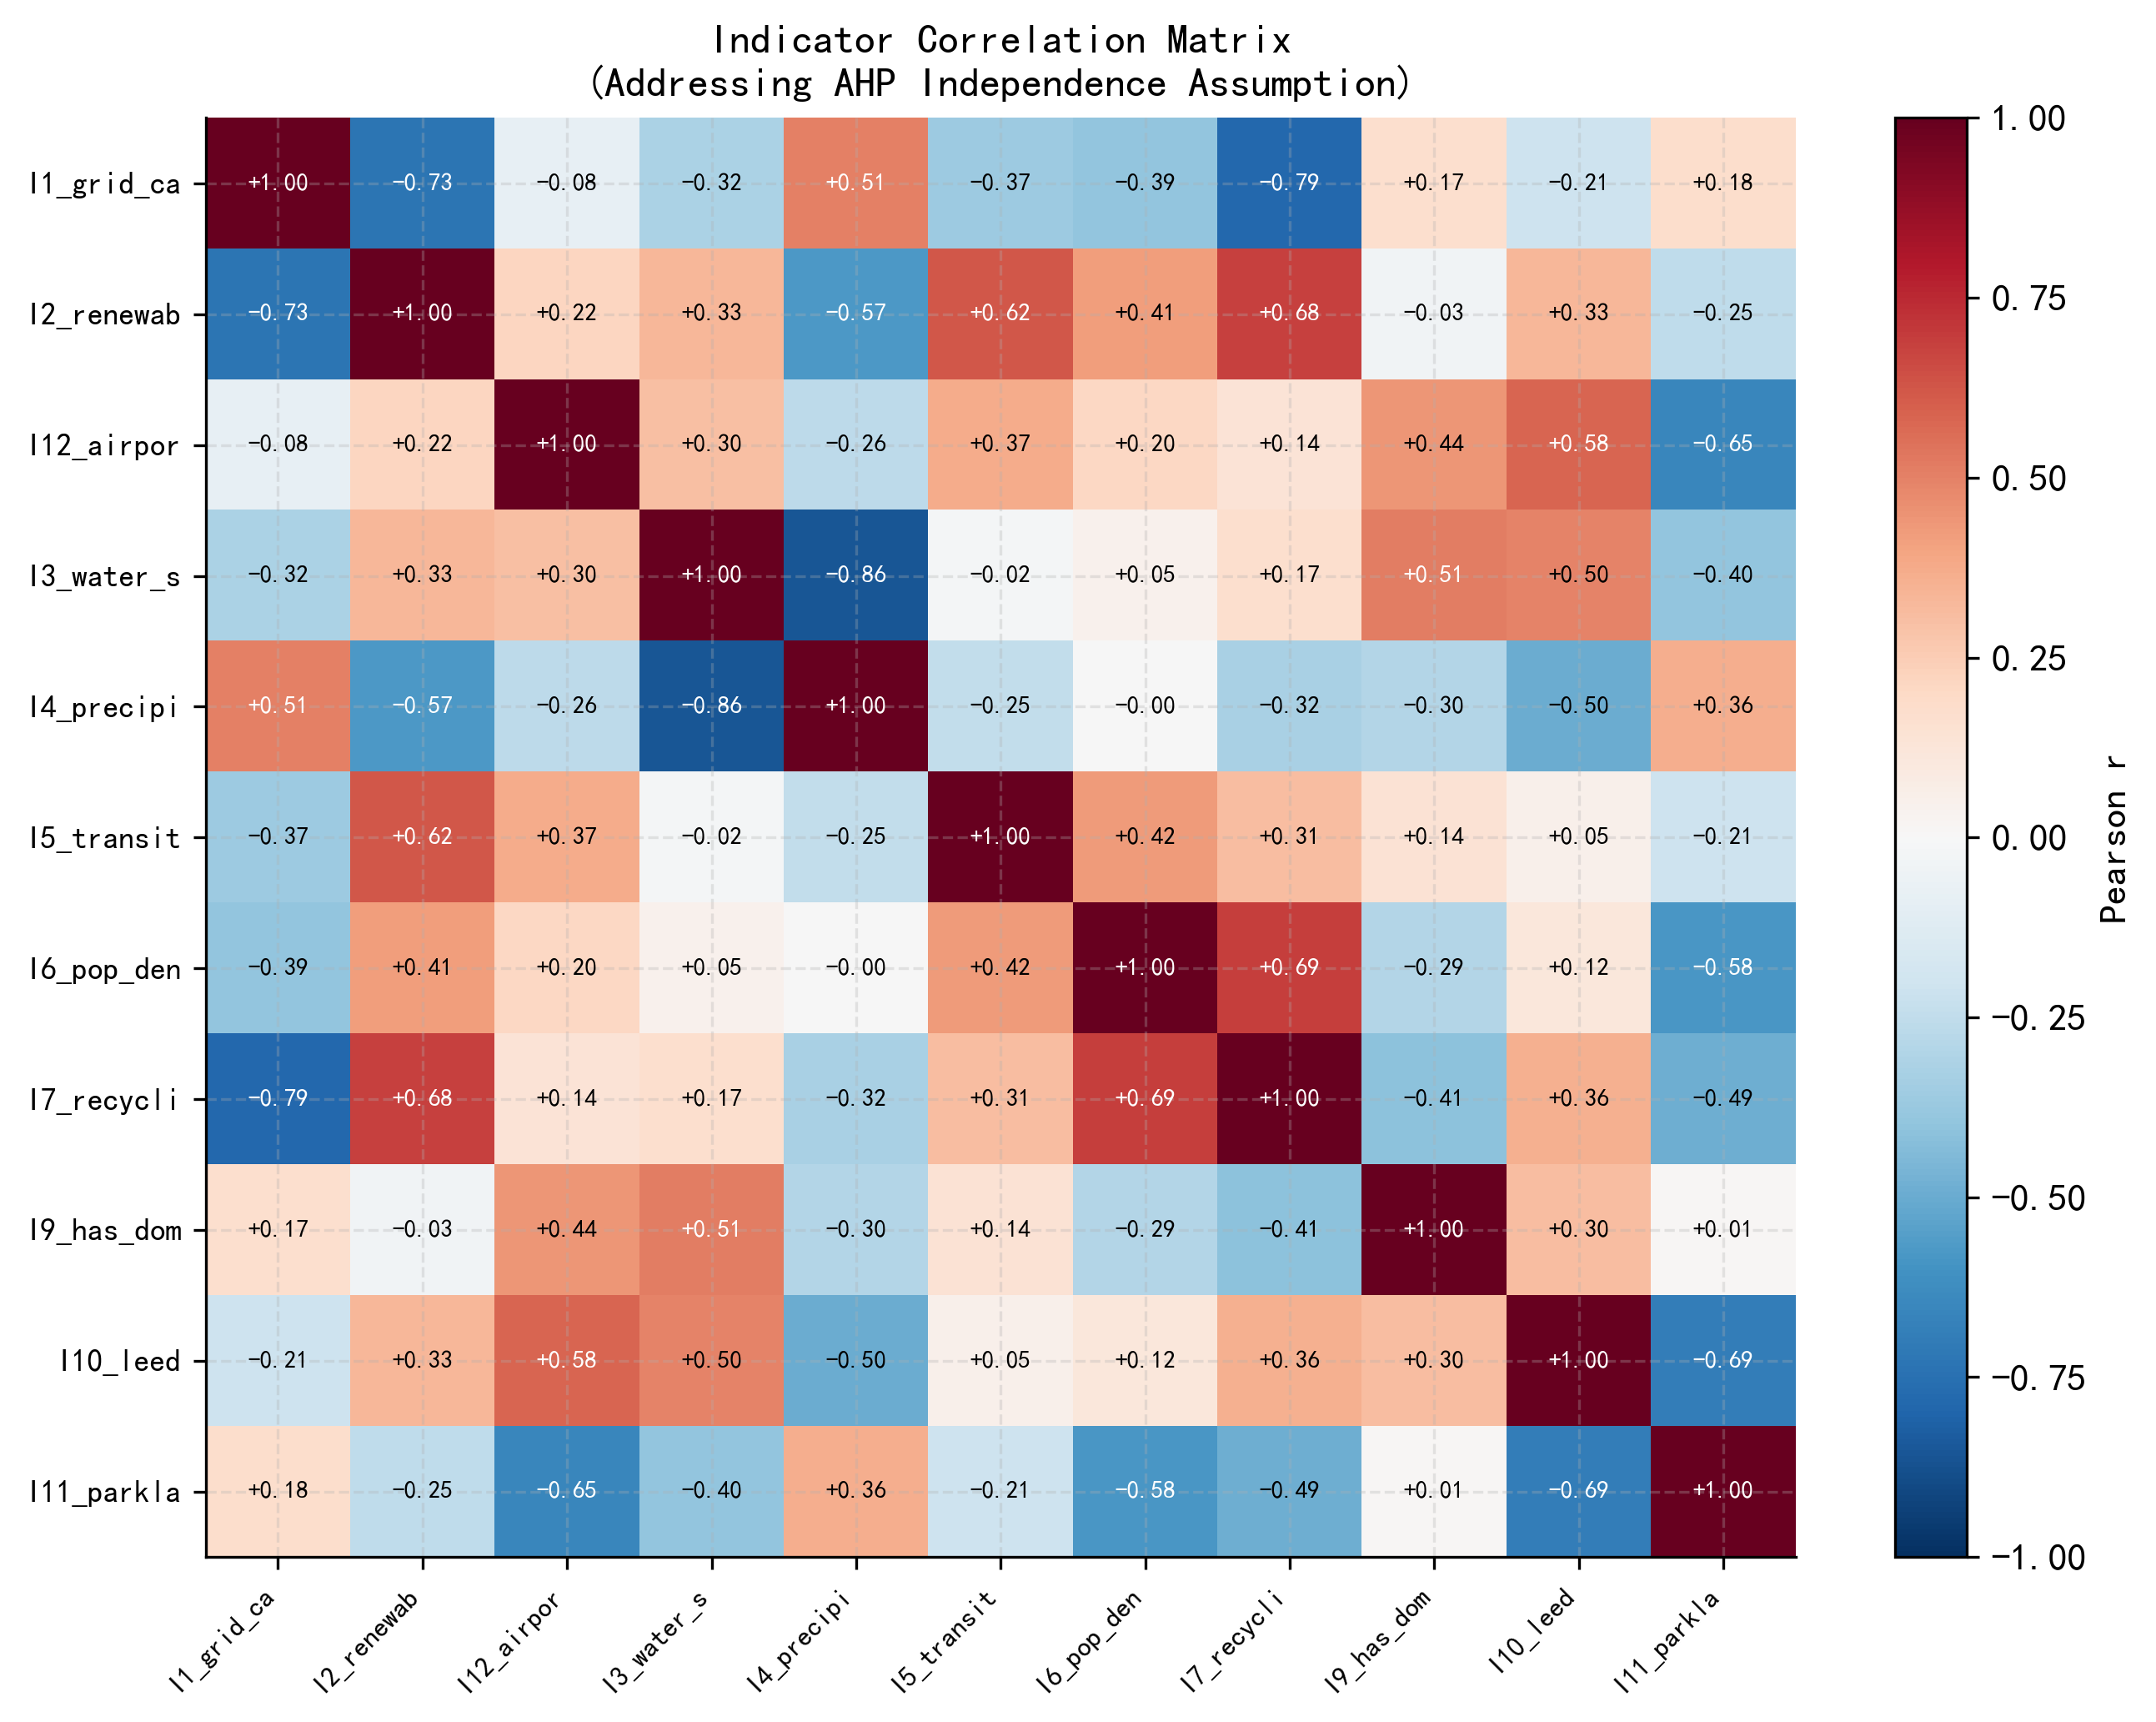
\includegraphics[width=0.72\textwidth]{fig_q2_correlation_matrix.png}
\caption{12项指标Pearson相关系数矩阵}\label{fig:q2_correlation}
\end{figure}

\subsubsection{全局权重}

准则权重：C1（38.87\%）$>$ C3（25.58\%）$>$ C5（14.49\%）$>$ C2（8.58\%）$>$ C4（7.00\%）$>$ C6（5.47\%）。

\begin{table}[H]
\centering
\caption{12指标全局权重（主特征向量法，4位小数，回应L8）}
\label{tab:global_weights}
\begin{tabular}{clccc}
\toprule
\textbf{编号} & \textbf{指标} & \textbf{准则} & \textbf{权重（\%）} & \textbf{方向} \\
\midrule
I1  & 电网碳排放因子（kgCO$_2$/kWh） & C1 & 29.15 & 成本型 \\
I5  & 公共交通分担率（\%） & C3 & 15.99 & 效益型 \\
I2  & 可再生能源占比（\%） & C1 & 9.72 & 效益型 \\
I9  & 体育场穹顶状态（0/1） & C5 & 9.66 & 效益型 \\
I7  & 废物回收率（\%） & C4 & 7.00 & 效益型 \\
I3  & 水资源压力指数（WRI） & C2 & 6.43 & 成本型 \\
I6  & 人口密度（每平方英里） & C3 & 6.10 & 效益型 \\
I8  & 二月温度适宜度 & C5 & 4.83 & 效益型 \\
I10 & 体育场LEED等级（0-4） & C6 & 4.11 & 效益型 \\
I12 & 机场旅客吞吐量（百万） & C3 & 3.49 & 成本型 \\
I4  & 年降水量（英寸） & C2 & 2.14 & 成本型 \\
I11 & 城市绿地面积占比（\%） & C6 & 1.37 & 效益型 \\
\bottomrule
\end{tabular}
\par\vspace{0.3em}\footnotesize
权重和为100.00\%（特征向量归一化的自然结果，非人为凑整）。
I12归属C3、方向为成本型（修正后）。
\end{table}

\begin{figure}[H]
\centering
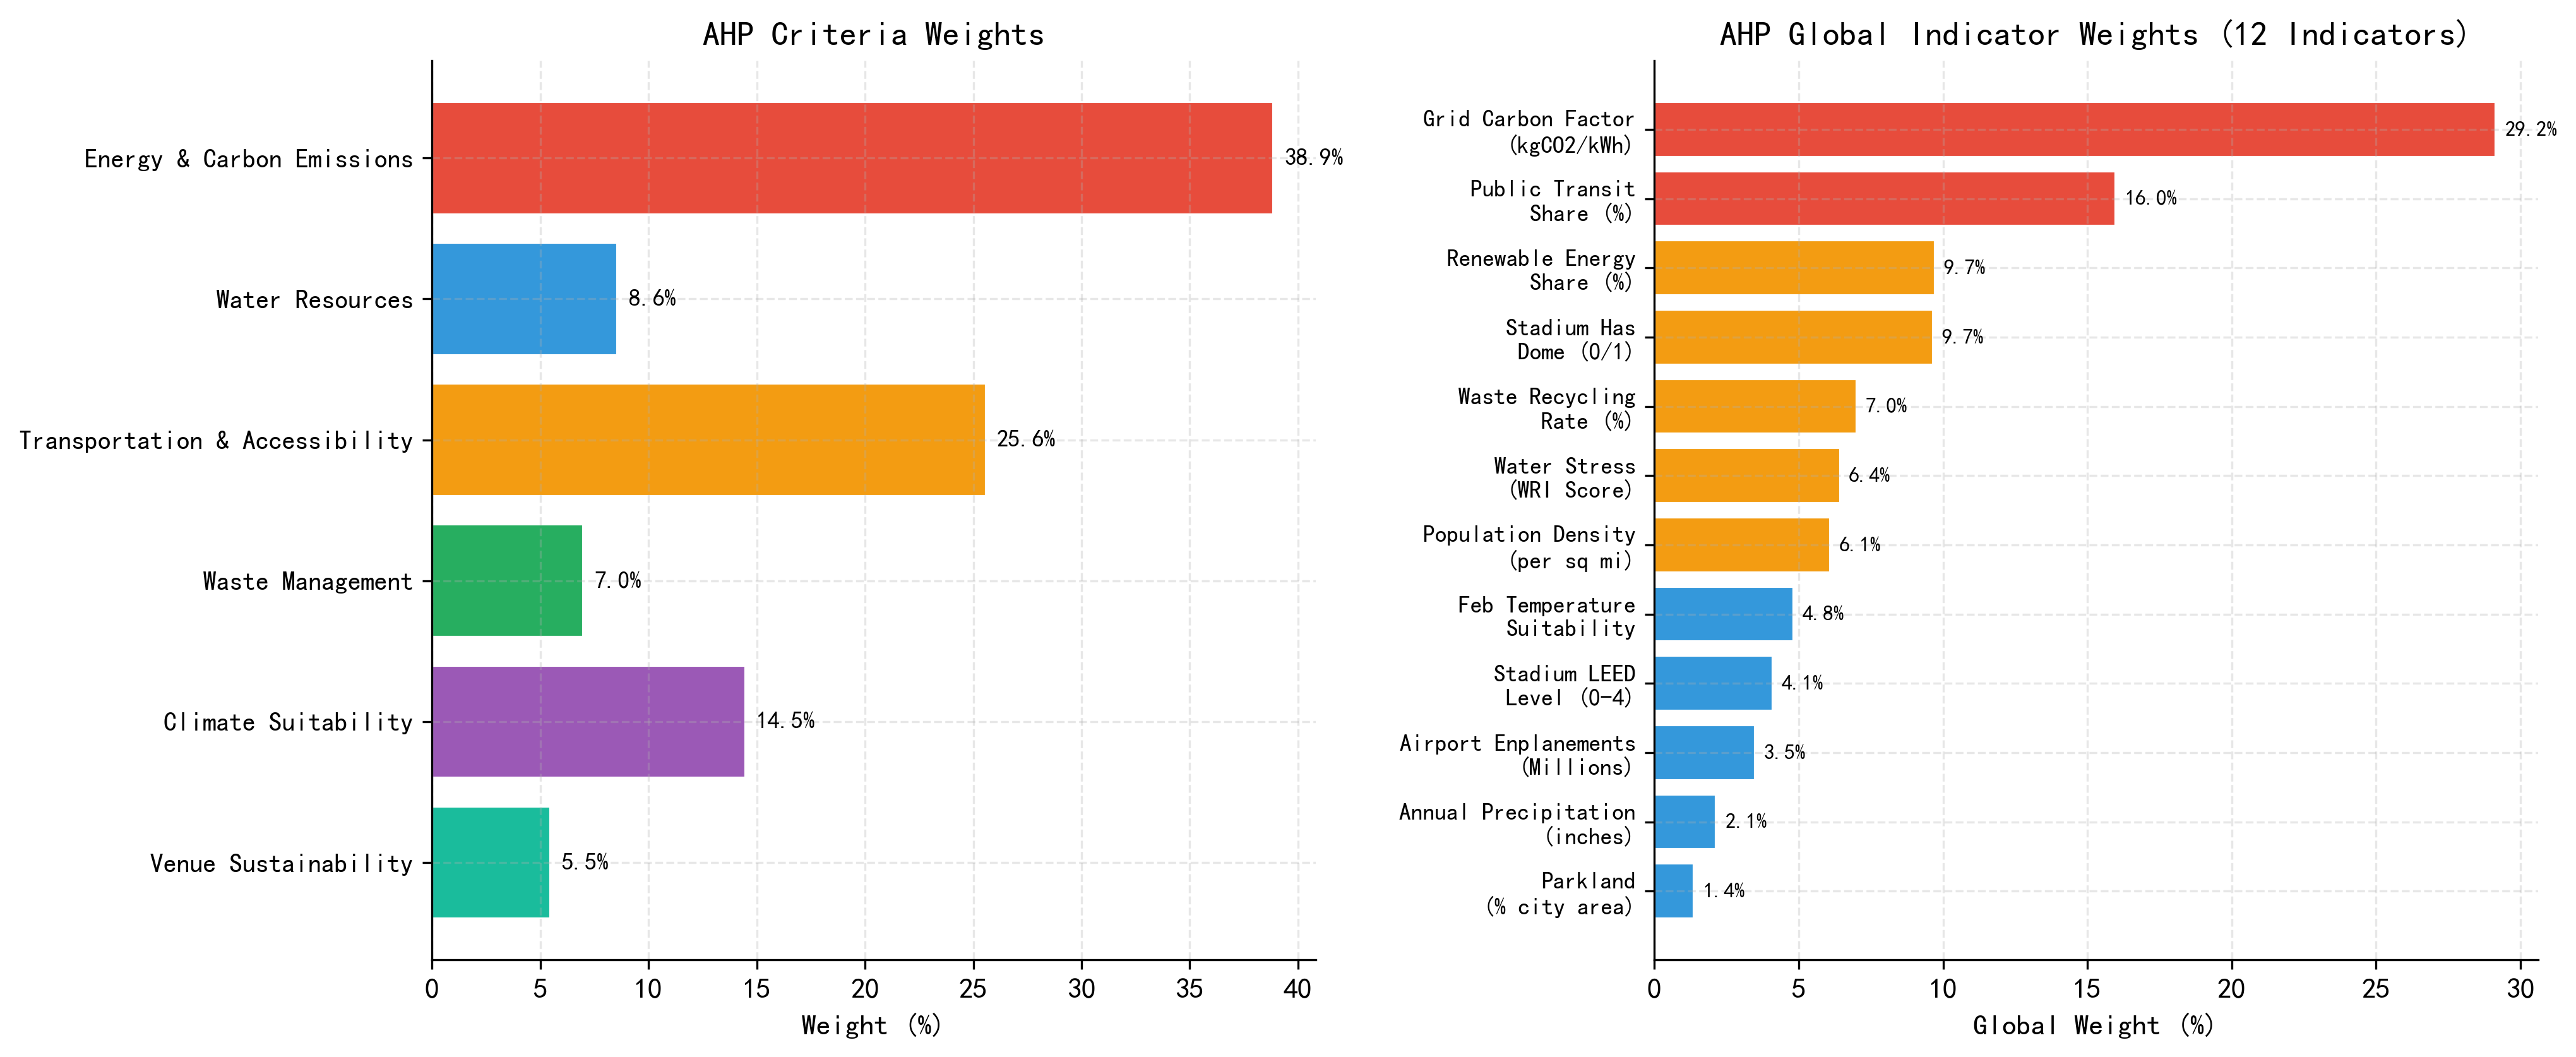
\includegraphics[width=0.90\textwidth]{fig_q2_ahp_weights.png}
\caption{AHP权重：准则层（左）与12指标全局权重排序（右）}\label{fig:q2_weights}
\end{figure}

\subsection{问题三a：已办城市TOPSIS排序}\label{sec:q3a}

\subsubsection{TOPSIS模型}

\textbf{向量归一化} $r_{ij}=x_{ij}/\sqrt{\sum_k x_{kj}^2}$；\textbf{加权} $v_{ij}=w_j r_{ij}$；
\textbf{理想解} $A^+=\{ \max_i v_{ij}\mid j\in J_{\text{benefit}};\ \min_i v_{ij}\mid j\in J_{\text{cost}} \}$，
$A^-$取反向极值；
\textbf{欧氏距离} $D_i^\pm=\sqrt{\sum_j(v_{ij}-v_j^\pm)^2}$；
\textbf{贴近度} $C_i=D_i^-/(D_i^++D_i^-)$。

\textbf{温度适宜度公式修正（回应M5）}：
\begin{equation}
S_{\text{temp},i} =
\begin{cases}
9.0, & \text{若 } \text{I9}_i = 1 \text{（穹顶体育场，气候受控）} \\
\max\left(0,\; 10 - |T_{\text{feb},i} - 18| \right), & \text{若 } \text{I9}_i = 0 \text{（露天体育场）}
\end{cases}
\end{equation}

修正理由：穹顶体育场内温度受气候控制系统调节，不应因城市室外温度受到惩罚；露天体育场下限截断为0，避免负分。三种方案对比见表\ref{tab:temp_robustness}（三种方案下西雅图排名一致，结论稳健）。

\begin{table}[H]
\centering
\caption{温度公式稳健性对比}
\label{tab:temp_robustness}
\small
\begin{tabular}{lccc}
\toprule
\textbf{方案} & \textbf{穹顶体育场} & \textbf{露天体育场} & \textbf{西雅图排名} \\
\midrule
(a) $10-|T-18|$（旧） & 与露天相同 & 可产生负分 & 第1（13城） \\
(b) $\max(0,10-|T-18|)$ & 与露天相同 & 截断为0 & 第1 \\
(c) 穹顶9分, 露天截断（采用） & 固定9分 & 截断为0 & 第1 \\
\bottomrule
\end{tabular}
\end{table}

\subsubsection{10城排序结果}

\begin{table}[H]
\centering
\caption{10个已办城市TOPSIS排序（回应H1更新值）}
\label{tab:q3a_ranking}
\begin{tabular}{ccccc}
\toprule
\textbf{排名} & \textbf{城市} & \textbf{贴近度$C_i$} & $D_i^{+}$ & $D_i^{-}$ \\
\midrule
1 & 英格尔伍德（洛杉矶） & 0.7637 & 0.0293 & 0.0949 \\
2 & 圣克拉拉 & 0.6160 & 0.0519 & 0.0832 \\
3 & 拉斯维加斯 & 0.5271 & 0.0585 & 0.0652 \\
4 & 休斯顿 & 0.4834 & 0.0639 & 0.0598 \\
5 & 达拉斯（阿灵顿） & 0.4559 & 0.0656 & 0.0549 \\
6 & 格兰岱尔（凤凰城） & 0.4471 & 0.0715 & 0.0579 \\
7 & 亚特兰大 & 0.4302 & 0.0782 & 0.0590 \\
8 & 迈阿密（迈阿密花园） & 0.3961 & 0.0773 & 0.0507 \\
9 & 新奥尔良 & 0.3853 & 0.0828 & 0.0519 \\
10 & 坦帕 & 0.2774 & 0.0886 & 0.0340 \\
\bottomrule
\end{tabular}
\end{table}

英格尔伍德以$C=0.7637$排名第一（领先圣克拉拉23.9\%）。其优势：CAMX电网因子0.226 kgCO$_2$/kWh（最低）、51\%可再生能源、SoFi体育场LEED金级+ETFE穹顶。坦帕垫底：FRCC电网因子0.369 kgCO$_2$/kWh、8\%可再生能源、无穹顶、公交分担率1.7\%。

\begin{figure}[H]
\centering
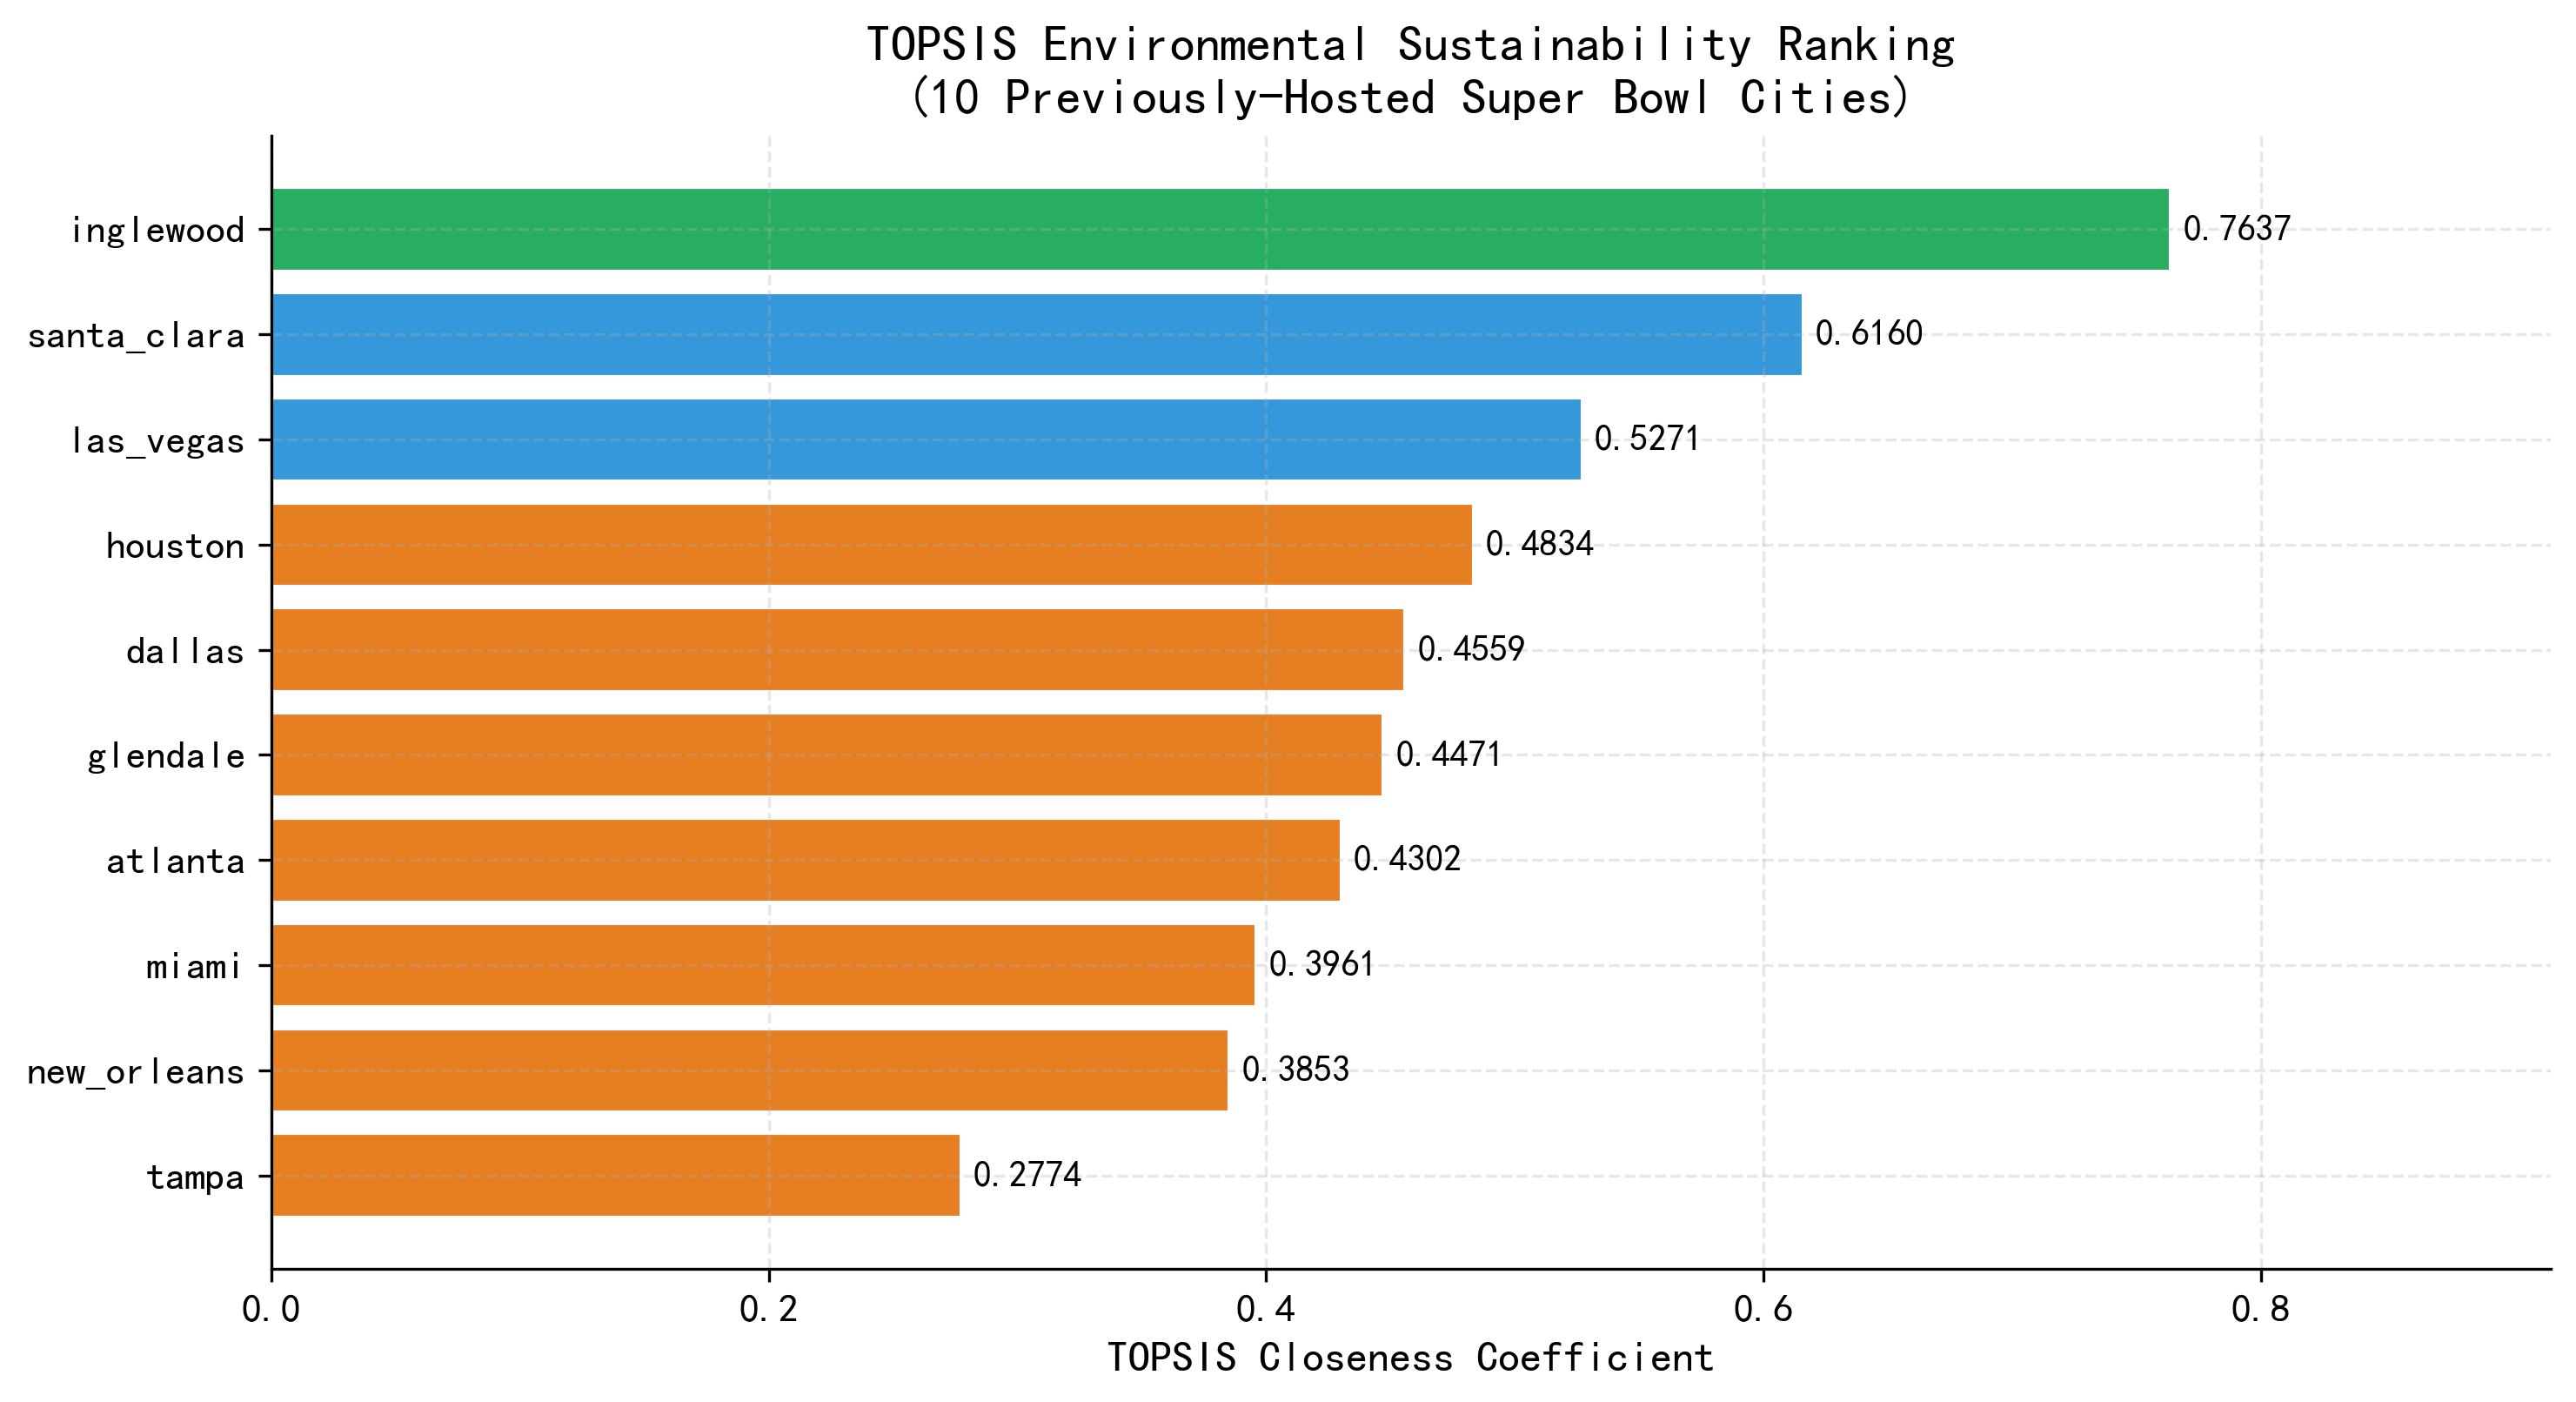
\includegraphics[width=0.85\textwidth]{fig_q3a_topsis_ranking.png}
\caption{10城TOPSIS环境可持续排名}\label{fig:q3a_ranking}
\end{figure}

\subsubsection{TOPSIS集合依赖性与排名逆转分析（回应M4）}

TOPSIS的$C_i$值依赖评价集构成。英格尔伍德在10城排序中$C_{10}=0.7637$，13城合并中$C_{13}=0.6442$（变化非因表现变差，而是归一化基准变化）。

\textbf{加入西雅图后理想解的变化}：
\begin{itemize}[itemsep=0.1em]
  \item \textbf{I2（可再生能源）极值}：正理想解从英格尔伍德的51\%变为西雅图的69\%。西雅图将效益型指标的``天花板''提高了35\%，使所有其他城市在此指标上的相对得分降低。英格尔伍德在I2上的加权归一化值从$0.0102$（10城，占正理想解1.5\%）变为$0.0081$（13城）。
  \item \textbf{I3（水压力）极值}：正理想解（成本型取最小值）从新奥尔良的WRI 1.0变为西雅图的WRI 0.5。水资源维度上的竞争基准被显著提升。
  \item \textbf{I6（人口密度）极值}：西雅图以9,047人/平方英里成为该指标的新``最优''（正理想解，效益型），改变了城市形态维度的参照系。
  \item \textbf{I8（温度适宜度）范数}：10城与13城范数比仅为0.7203（见表\ref{tab:set_dependency}），是范数收缩最大的指标——因为穹顶城市在修正公式下得分9.0（全城最高），而西雅图（露天，6.3$^\circ$C$\to$0分）大幅拉低了该指标的均值和范数。
\end{itemize}

\textbf{排名逆转的本质}：并非西雅图在所有指标上全面优于英格尔伍德（实际上英格尔伍德的穹顶、LEED和机场得分更高），而是西雅图在I2（权重9.7\%）、I3（6.4\%）、I6（6.1\%）三个效益型指标上的极值同时改变，累积效应超过了英格尔伍德在I9（穹顶权重9.7\%）上的优势。这体现了TOPSIS的集合依赖性——新方案的加入可同时改变多个指标的理想解。

\begin{table}[H]
\centering
\caption{集合依赖性：10城 vs 13城 指标范数比较}
\label{tab:set_dependency}
\small
\begin{tabular}{lccc}
\toprule
\textbf{指标} & \textbf{$\mathcal{N}_{10}$} & \textbf{$\mathcal{N}_{13}$} & \textbf{比率} \\
\midrule
I2 可再生能源 & 95.02 & 118.97 & 1.25 \\
I5 公交分担率 & 9.30 & 11.38 & 1.22 \\
I8 温度适宜度 & 26.80 & 19.31 & 0.72 \\
I1 电网碳 & 1.09 & 1.23 & 1.13 \\
\bottomrule
\end{tabular}
\par\vspace{0.3em}\footnotesize
$\mathcal{N}_j=\sqrt{\sum x_{ij}^2}$为向量归一化分母。比率$>$1表示范数增大（加入新城市后参考基准扩展），$<$1表示范数收缩。
\end{table}

\textbf{对照实验}：剔除西雅图的12城排序中英格尔伍德回归第一（$C_{12}=0.7615$），说明西雅图的真实竞争力而非范数变化是排位重组的主因。

\subsection{问题三b：未办城市合并排序}\label{sec:q3b}

\begin{table}[H]
\centering
\caption{13城合并TOPSIS排序}
\label{tab:q3b_combined}
\begin{tabular}{cccccc}
\toprule
\textbf{排名} & \textbf{城市} & \textbf{已办？} & \textbf{$C_i$} & $D_i^{+}$ & $D_i^{-}$ \\
\midrule
1 & 西雅图 & 否 & 0.6558 & 0.0507 & 0.0966 \\
2 & 英格尔伍德 & 是 & 0.6442 & 0.0474 & 0.0858 \\
3 & 圣克拉拉 & 是 & 0.5195 & 0.0673 & 0.0727 \\
4 & 拉斯维加斯 & 是 & 0.4710 & 0.0690 & 0.0614 \\
5 & 休斯顿 & 是 & 0.4431 & 0.0724 & 0.0576 \\
6 & 格兰岱尔 & 是 & 0.4185 & 0.0777 & 0.0559 \\
7 & 亚特兰大 & 是 & 0.4176 & 0.0823 & 0.0590 \\
8 & 达拉斯 & 是 & 0.4119 & 0.0761 & 0.0533 \\
9 & 新奥尔良 & 是 & 0.3674 & 0.0906 & 0.0526 \\
10 & 迈阿密 & 是 & 0.3597 & 0.0871 & 0.0489 \\
11 & 夏洛特 & 否 & 0.3588 & 0.0852 & 0.0477 \\
12 & 坦帕 & 是 & 0.2621 & 0.0990 & 0.0352 \\
13 & 纳什维尔 & 否 & 0.2107 & 0.1080 & 0.0288 \\
\bottomrule
\end{tabular}
\end{table}

西雅图优势：69\%可再生能源（水电）、NWPP电网0.273 kgCO$_2$/kWh、56\%废物回收率、5.7\%公交分担率、WRI 0.5水压力（极低）。纳什维尔垫底（$C=0.2107$）：SRTV高碳电网（0.423 kgCO$_2$/kWh）、13\%可再生能源、1.5\%公交、无穹顶露天体育场。

\begin{figure}[H]
\centering
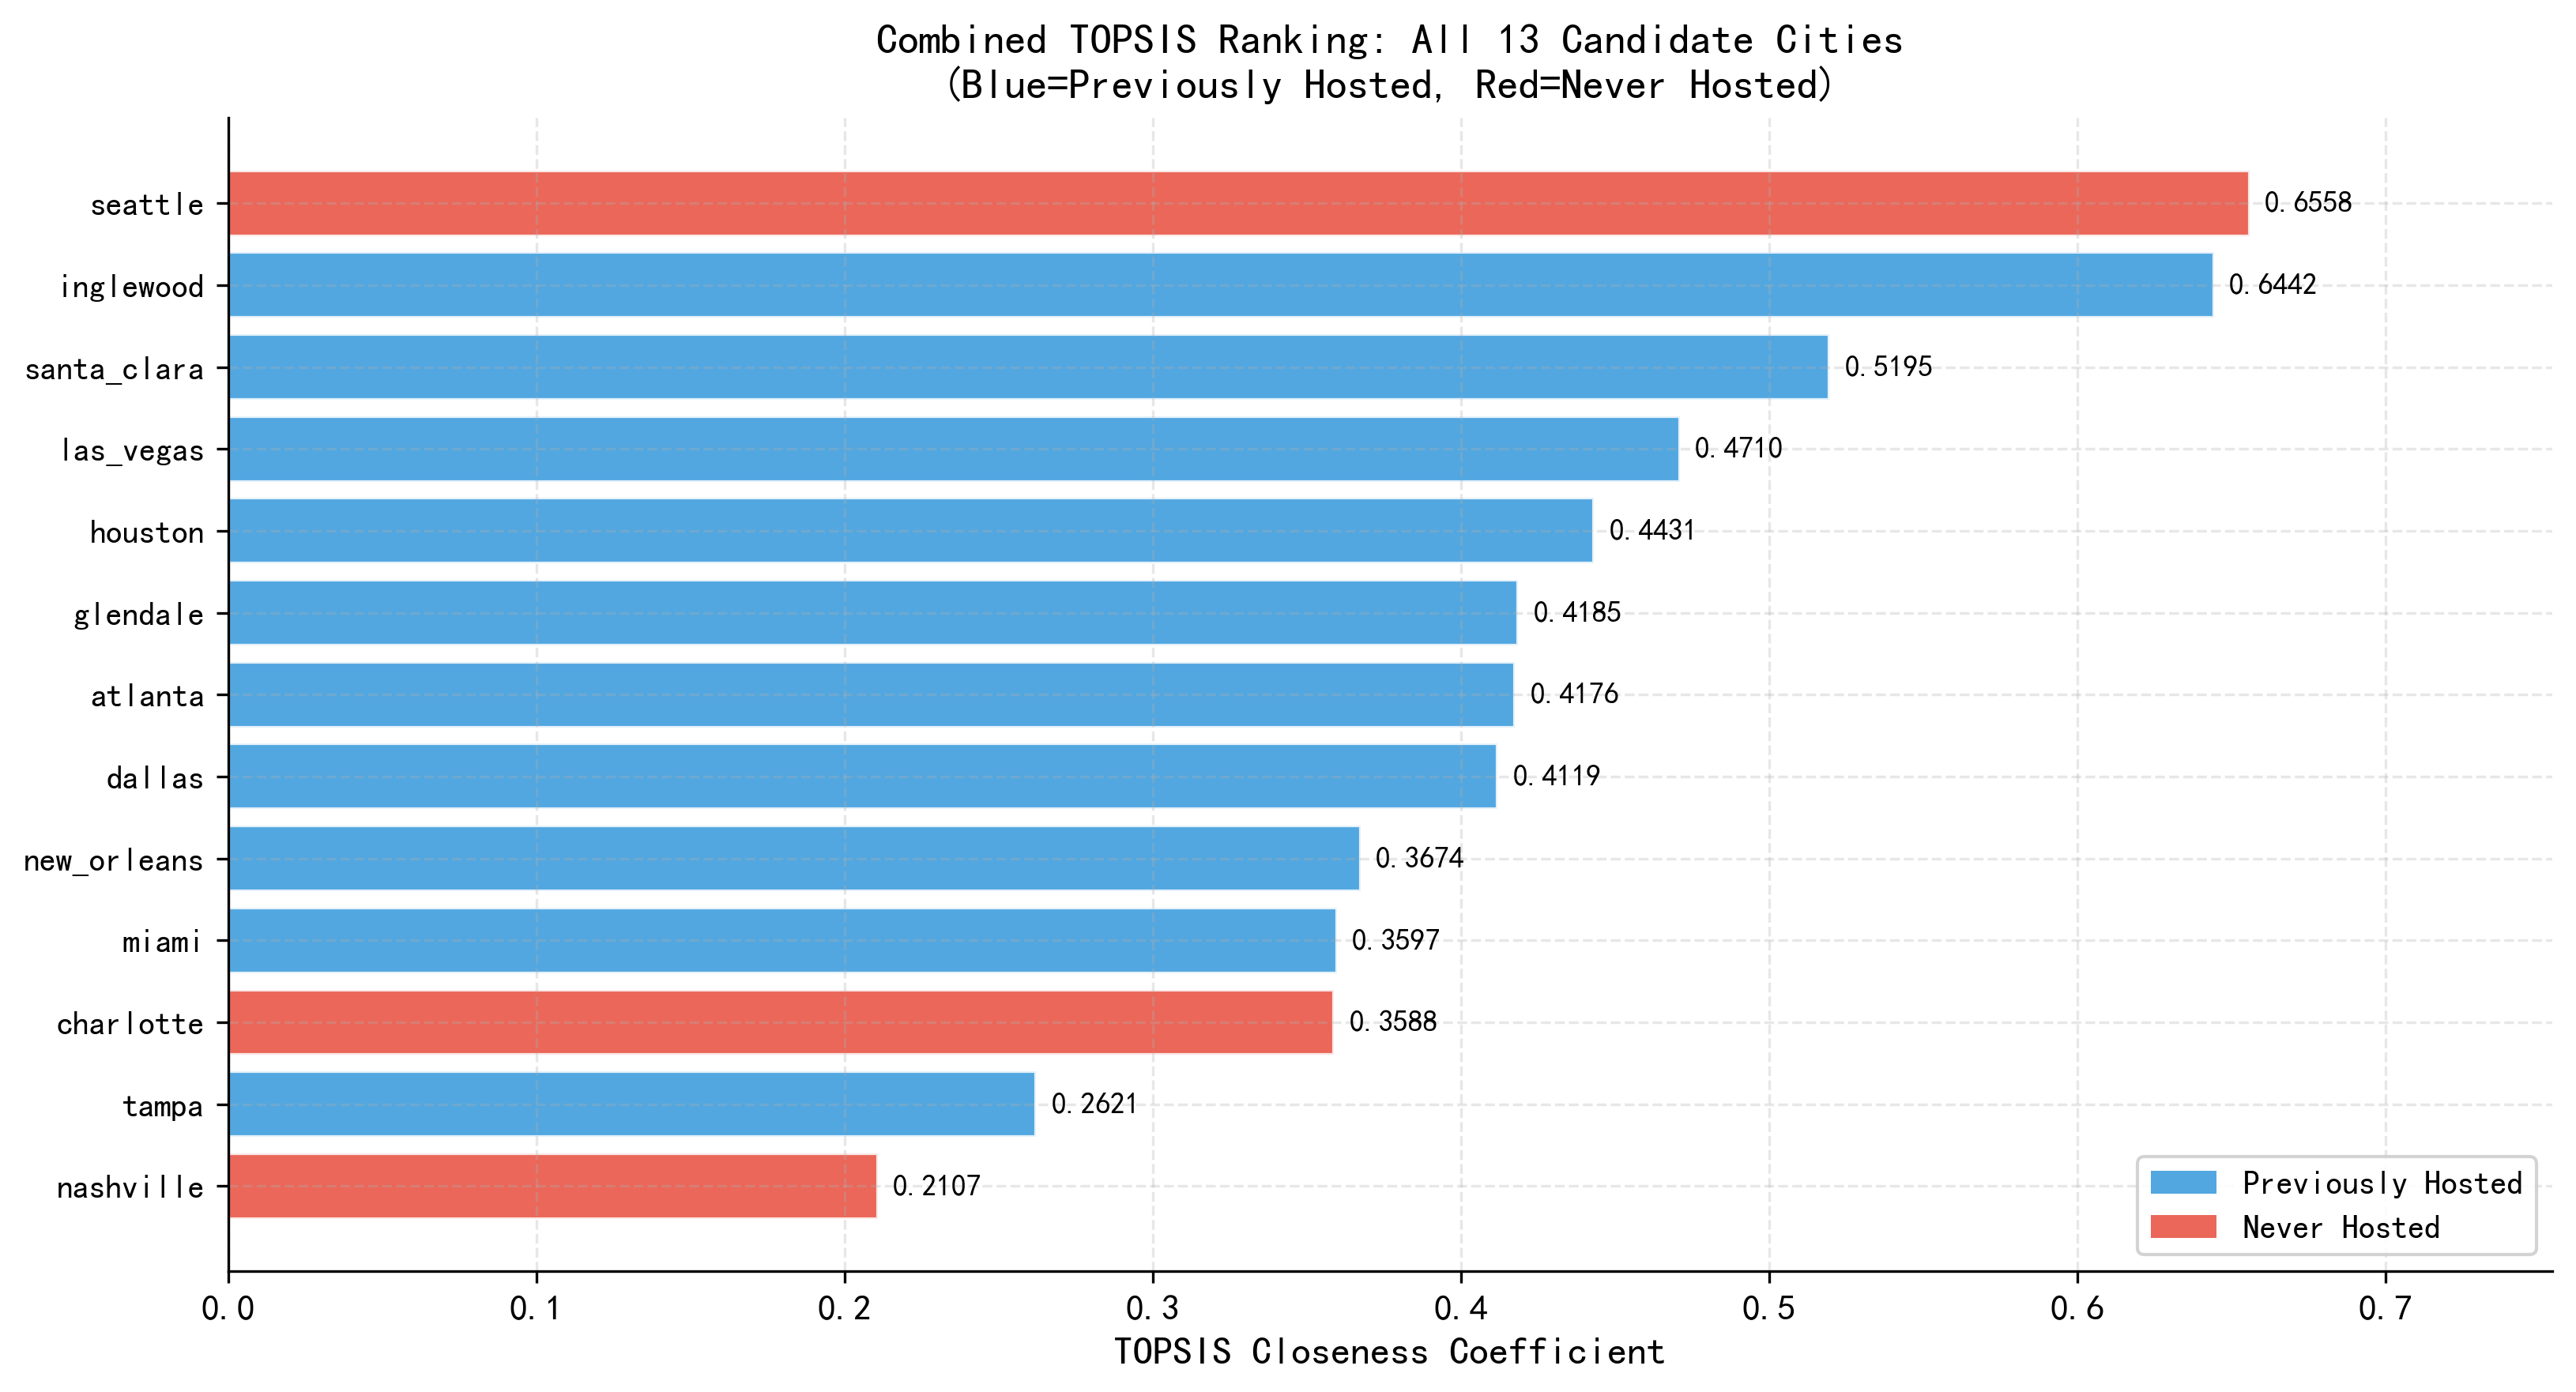
\includegraphics[width=0.88\textwidth]{fig_q3b_combined_ranking.png}
\caption{13城合并TOPSIS排序（蓝=已办，红=未办）}\label{fig:q3b_combined}
\end{figure}

\subsection{问题四a-b：扩展模型与奥运会应用}\label{sec:q4ab}

\subsubsection{模型扩展（4a）}
新增C7``多场馆物流''准则和4个奥运专属指标（I13场馆间距、I14运动员村可持续评分、I15临时材料占比、I16赛事天数），形成7准则16指标框架。7$\times$7准则矩阵$\lambda_{\max}=7.177$，CR=0.022，通过。温度适宜度改用7月平均温度、理想温度24$^\circ$C。

\subsubsection{2036年奥运会评估（4b）}
所有数据来自协调化国际数据库（IEA/EMBER/WRI/IRENA/Eurostat），缺失值标注插补方法。

\begin{table}[H]
\centering
\caption{2036年奥运会候选城市TOPSIS排序}
\label{tab:olympic_ranking}
\begin{tabular}{cccccc}
\toprule
\textbf{排名} & \textbf{城市} & \textbf{国家} & \textbf{$C_i$} & $D_i^{+}$ & $D_i^{-}$ \\
\midrule
1 & 伦敦 & 英国 & 0.7212 & 0.0605 & 0.1565 \\
2 & 马德里 & 西班牙 & 0.6750 & 0.0660 & 0.1370 \\
3 & 伊斯坦布尔 & 土耳其 & 0.6638 & 0.0699 & 0.1381 \\
4 & 柏林 & 德国 & 0.6033 & 0.0854 & 0.1298 \\
5 & 布里斯班 & 澳大利亚 & 0.5342 & 0.1117 & 0.1281 \\
6 & 艾哈迈达巴德 & 印度 & 0.3350 & 0.1455 & 0.0733 \\
7 & 多哈 & 卡塔尔 & 0.3123 & 0.1518 & 0.0690 \\
\bottomrule
\end{tabular}
\end{table}

伦敦优势：英国电网0.23 kgCO$_2$/kWh（IEA 2024）、48\%可再生能源（IRENA）、65\%回收率（Eurostat）、45\%公交分担率（TfL）、2012年奥运成熟基础设施。

\begin{figure}[H]
\centering
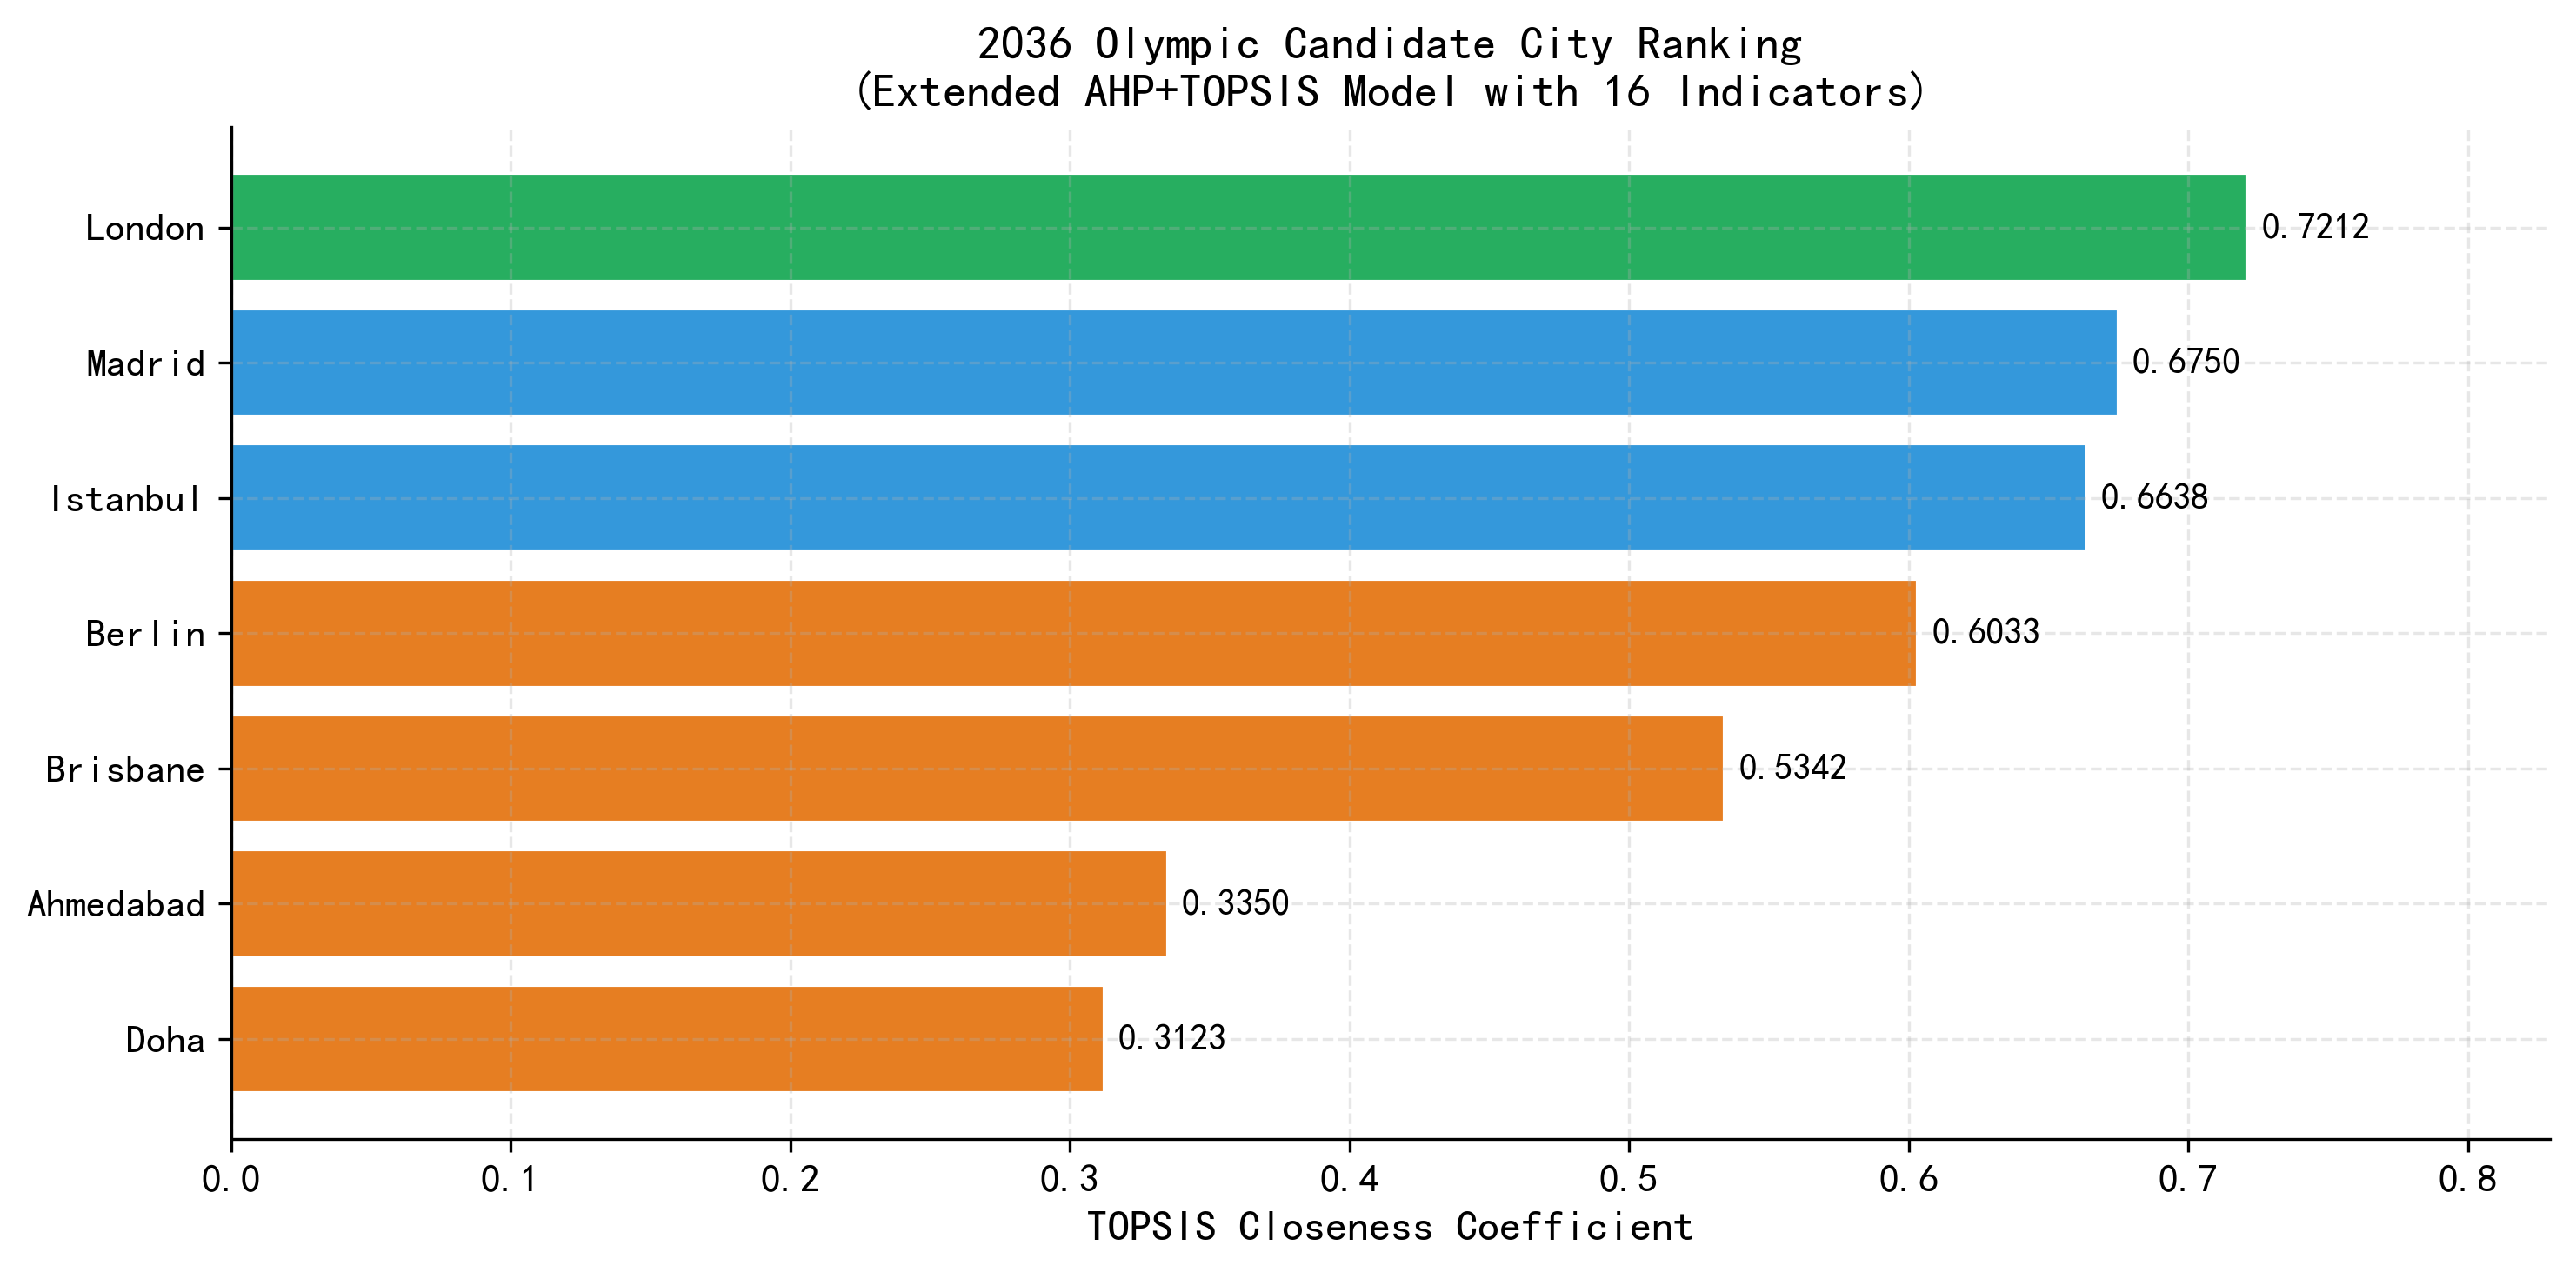
\includegraphics[width=0.88\textwidth]{fig_q4b_olympic_ranking.png}
\caption{2036年奥运会候选城市排序}\label{fig:q4b_ranking}
\end{figure}

\subsection{问题四c：情景分析}\label{sec:q4c}

四种情景：S0（基线）、S1（绿色能源：电网碳$-0.08$ kgCO$_2$/kWh，可再生$+15$pp）、S2（公交升级：公交分担$+5$pp）、S3（组合=S1+S2）。

\textbf{核心发现}：英格尔伍德各情景均第一（$\Delta C_{\text{max}}=+0.0068$），已达环境前沿。坦帕边际收益最大（S3下$\Delta C=+0.0299$）。亚特兰大组合策略下得分降低$\Delta C=-0.0202$——电网结构性劣势（0.423 kgCO$_2$/kWh）在归一化中被放大。

\begin{figure}[H]
\centering
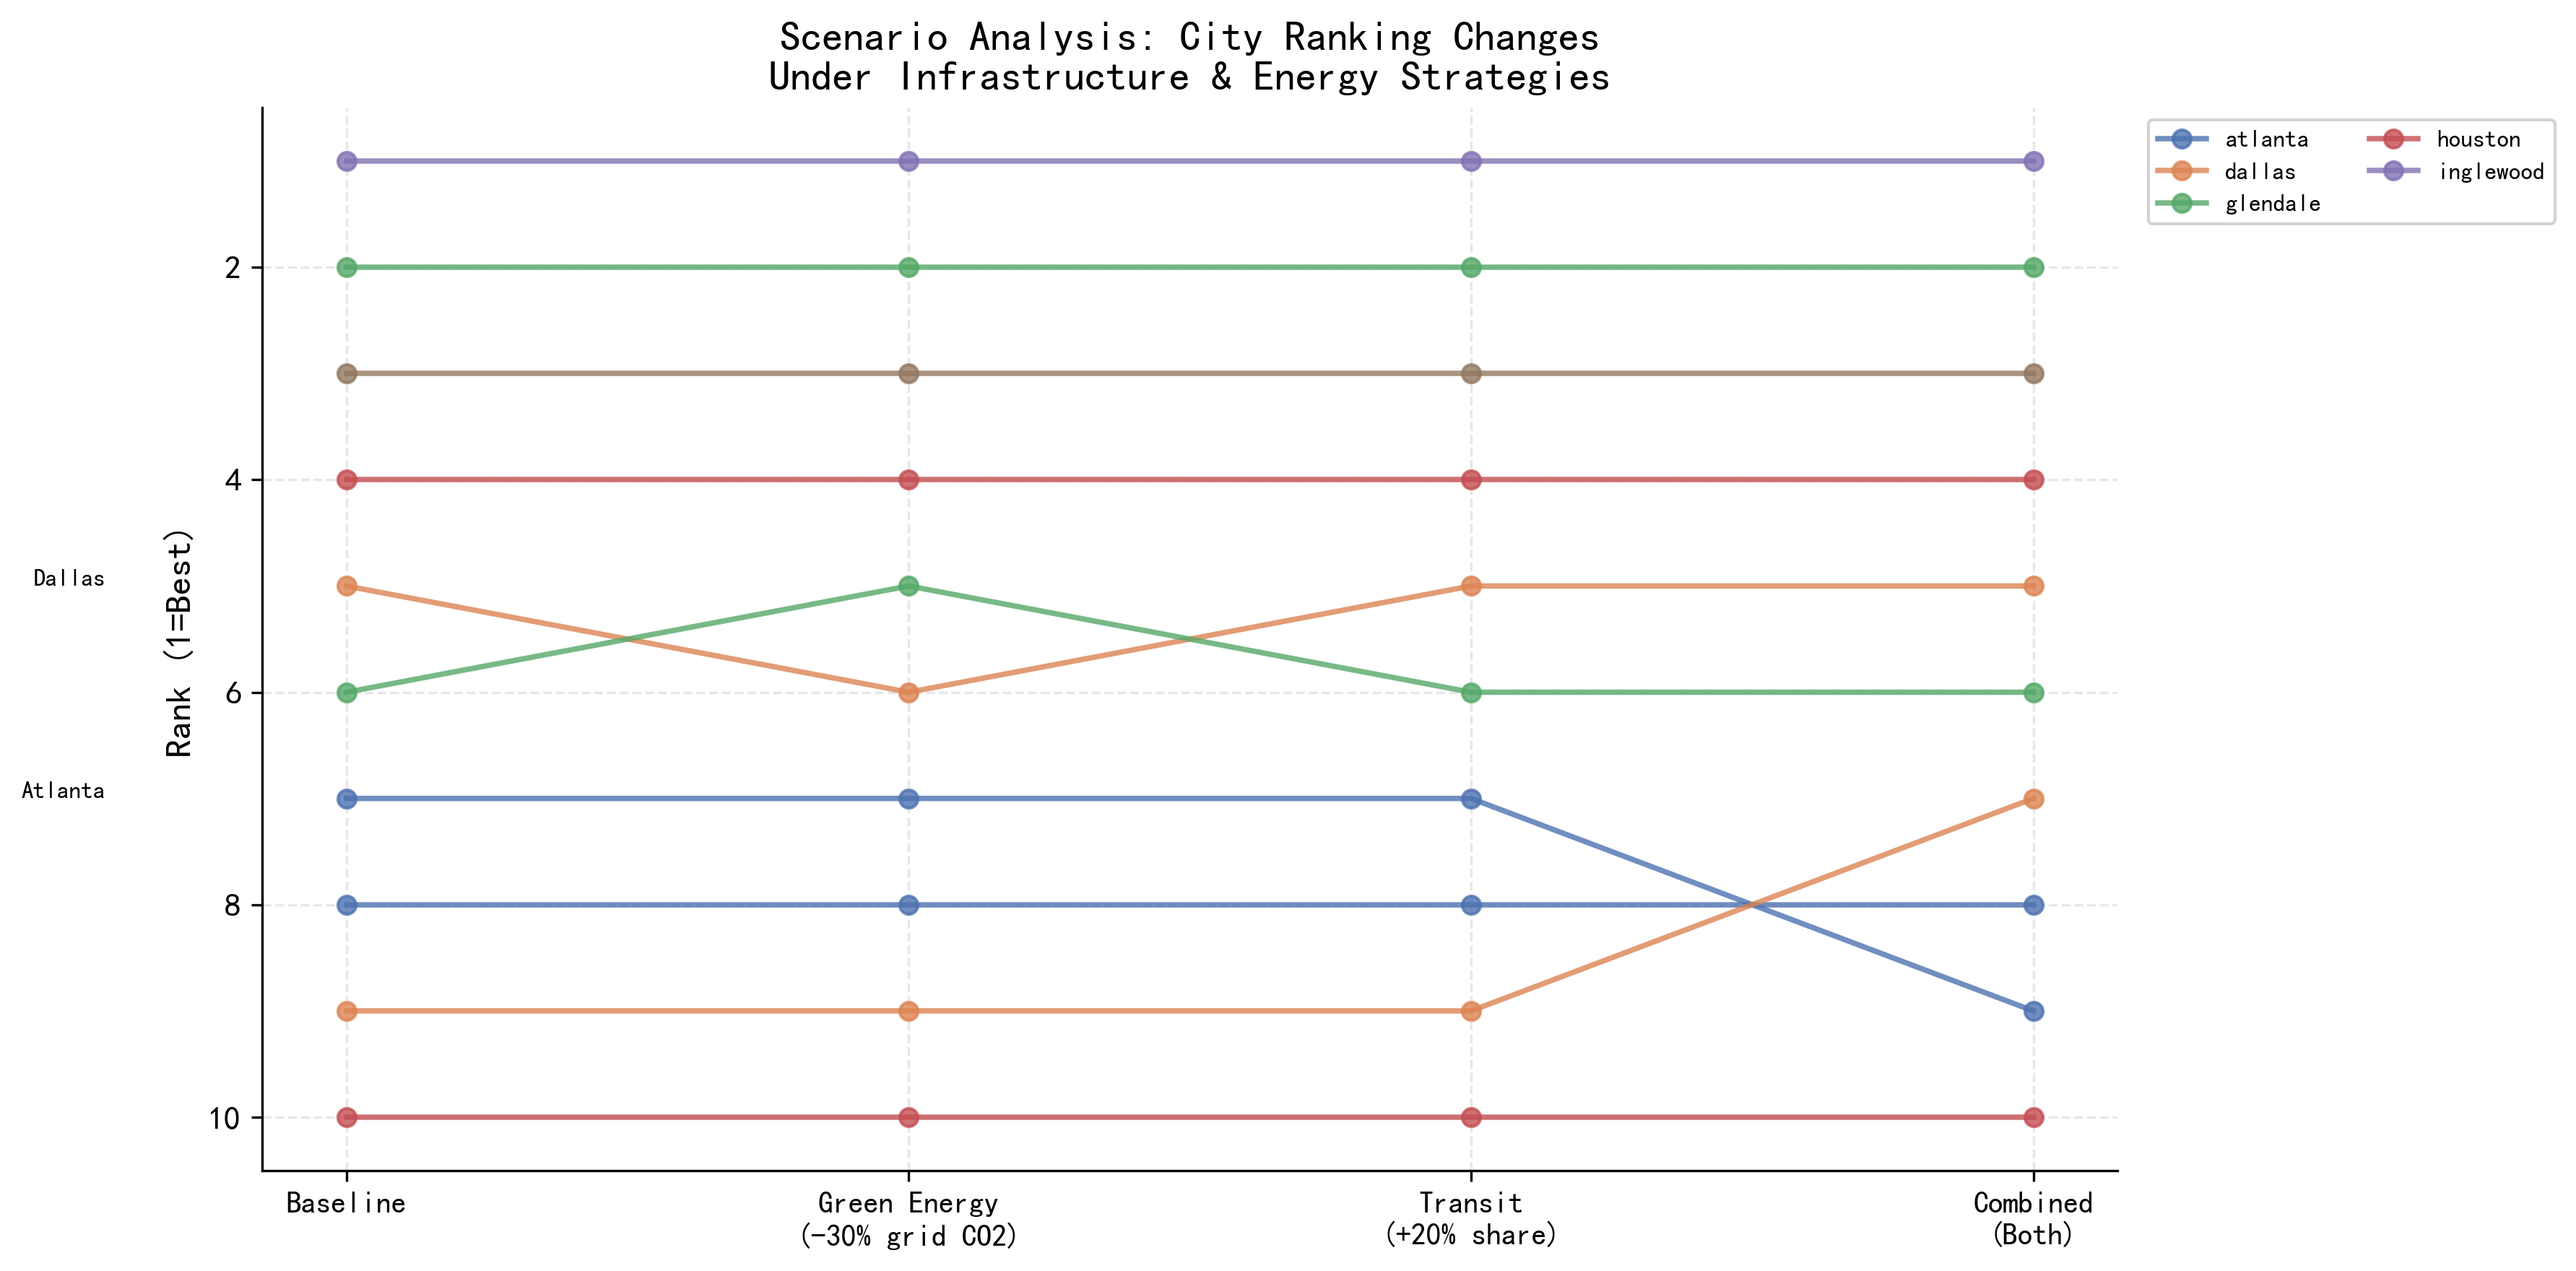
\includegraphics[width=0.85\textwidth]{fig_q4c_rank_changes.png}
\caption{四种情景下10城市排名变化}\label{fig:q4c_rank}
\end{figure}

\begin{figure}[H]
\centering
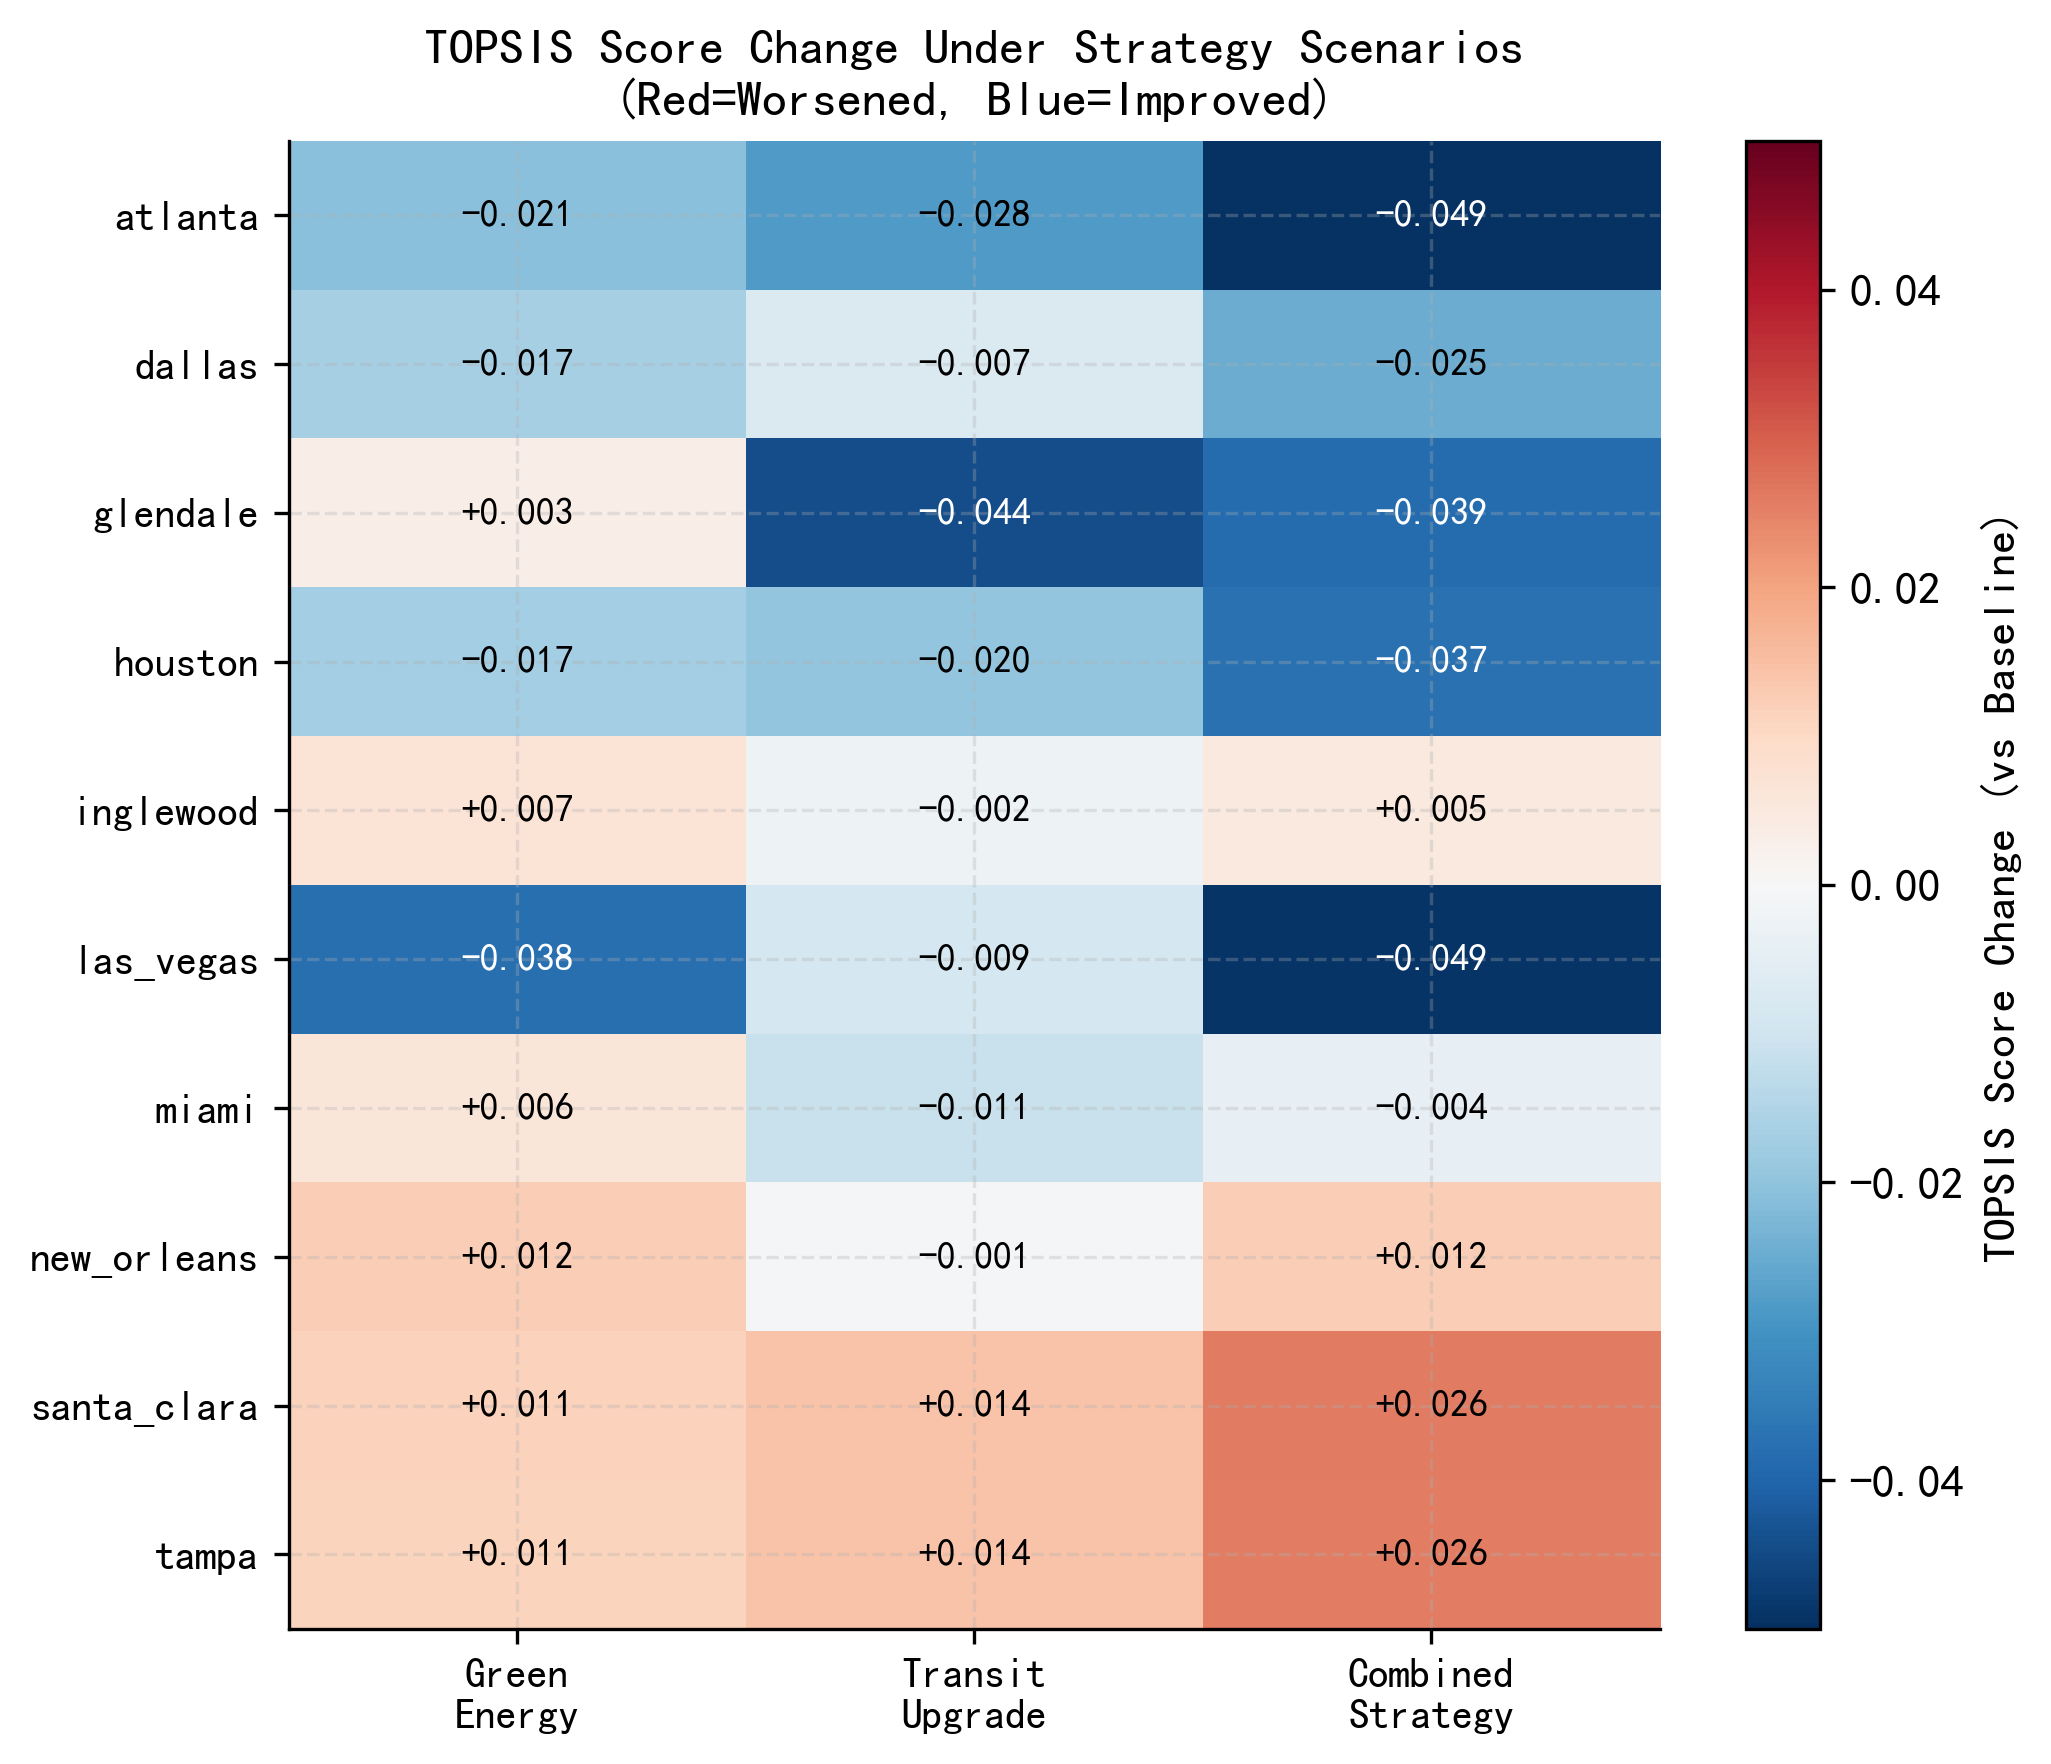
\includegraphics[width=0.78\textwidth]{fig_q4c_score_heatmap.png}
\caption{策略情景得分变化热力图（红=恶化，蓝=改善）}\label{fig:q4c_heatmap}
\end{figure}

\subsection{问题四d：超级碗vs奥运会碳排放结构对比}\label{sec:q4d}

\subsubsection{归一化定义与分母修正}

双归一化指标——每观众$\cdot$日强度$E_{\text{int}}^{\text{day}}$与每观众全程强度$E_{\text{int}}^{\text{event}}$。关键定义：总观众$\cdot$日 = 总售票数。奥运会800万总票数已是观众$\cdot$日的直接度量（每票=一个观众$\cdot$日）。

\subsubsection{排放数据来源（回应H2）}

\begin{table}[H]
\centering
\caption{碳排放参数——含来源与不确定范围（从数据文件读取）}
\label{tab:emission_params}
\small
\begin{tabular}{lccc}
\toprule
\textbf{参数} & \textbf{超级碗LIX} & \textbf{奥运会} & \textbf{来源} \\
\midrule
现场观众（总票数） & 65,000 & 800万 & NFL/官方售票 \\
赛事天数 & 1 & 17 & 赛程 \\
观众$\cdot$日 & 6.5万 & 800万 & =总票数 \\
总CO$_2$e（t） & \makecell[c]{100,000 \\ {[}75k--150k{]}}
  & \makecell[c]{3,500,000 \\ {[}2.5M--4.5M{]}}
  & \makecell[l]{SB: Jones(2018), Collins et al.(2009), \\ENGIE Impact(2024) \\
  Oly: IOC可持续报告, Cereceda et al.(2022)} \\
$E_{\text{int}}^{\text{day}}$ & \textbf{1,538} [1,154--2,308] & \textbf{438} [313--563] & — \\
\textbf{比值} & \multicolumn{2}{c}{\textbf{3.5倍} [2.1--7.4]} & — \\
Scope 3占比 & 75\% [70--80] & 66\% [58--75] &
  \makecell[l]{SB: Jones(2018); Oly: IOC报告} \\
\bottomrule
\end{tabular}
\end{table}

\textbf{超级碗排放计算方法论}：125,000访客 $\times$ 平均往返2,500英里 $\times$ 0.18 kgCO$_2$e/座位$\cdot$英里 $\approx$ 56,250 tCO$_2$e（Scope 3航空）。加上Scope 1（8k t）、Scope 2（17k t）、Scope 3住宿/其他（20k t），合计约100k tCO$_2$e[75k--150k]。奥运会取伦敦2012（3.3 Mt）、里约2016（3.6 Mt）、东京2020（2.7 Mt）中点3.5 Mt[2.5--4.5 Mt]\cite{IOC,Cereceda2022}。所有参数从`data/event\_emission\_params.csv`读取。

\textbf{更正说明}：初版将奥运会800万总票数误为唯一观众数后乘17天得虚假分母，导致60倍伪放大。更正后比值为3--4倍，反映超级碗单日飞行集中的真实结构性差异。

\begin{figure}[H]
\centering
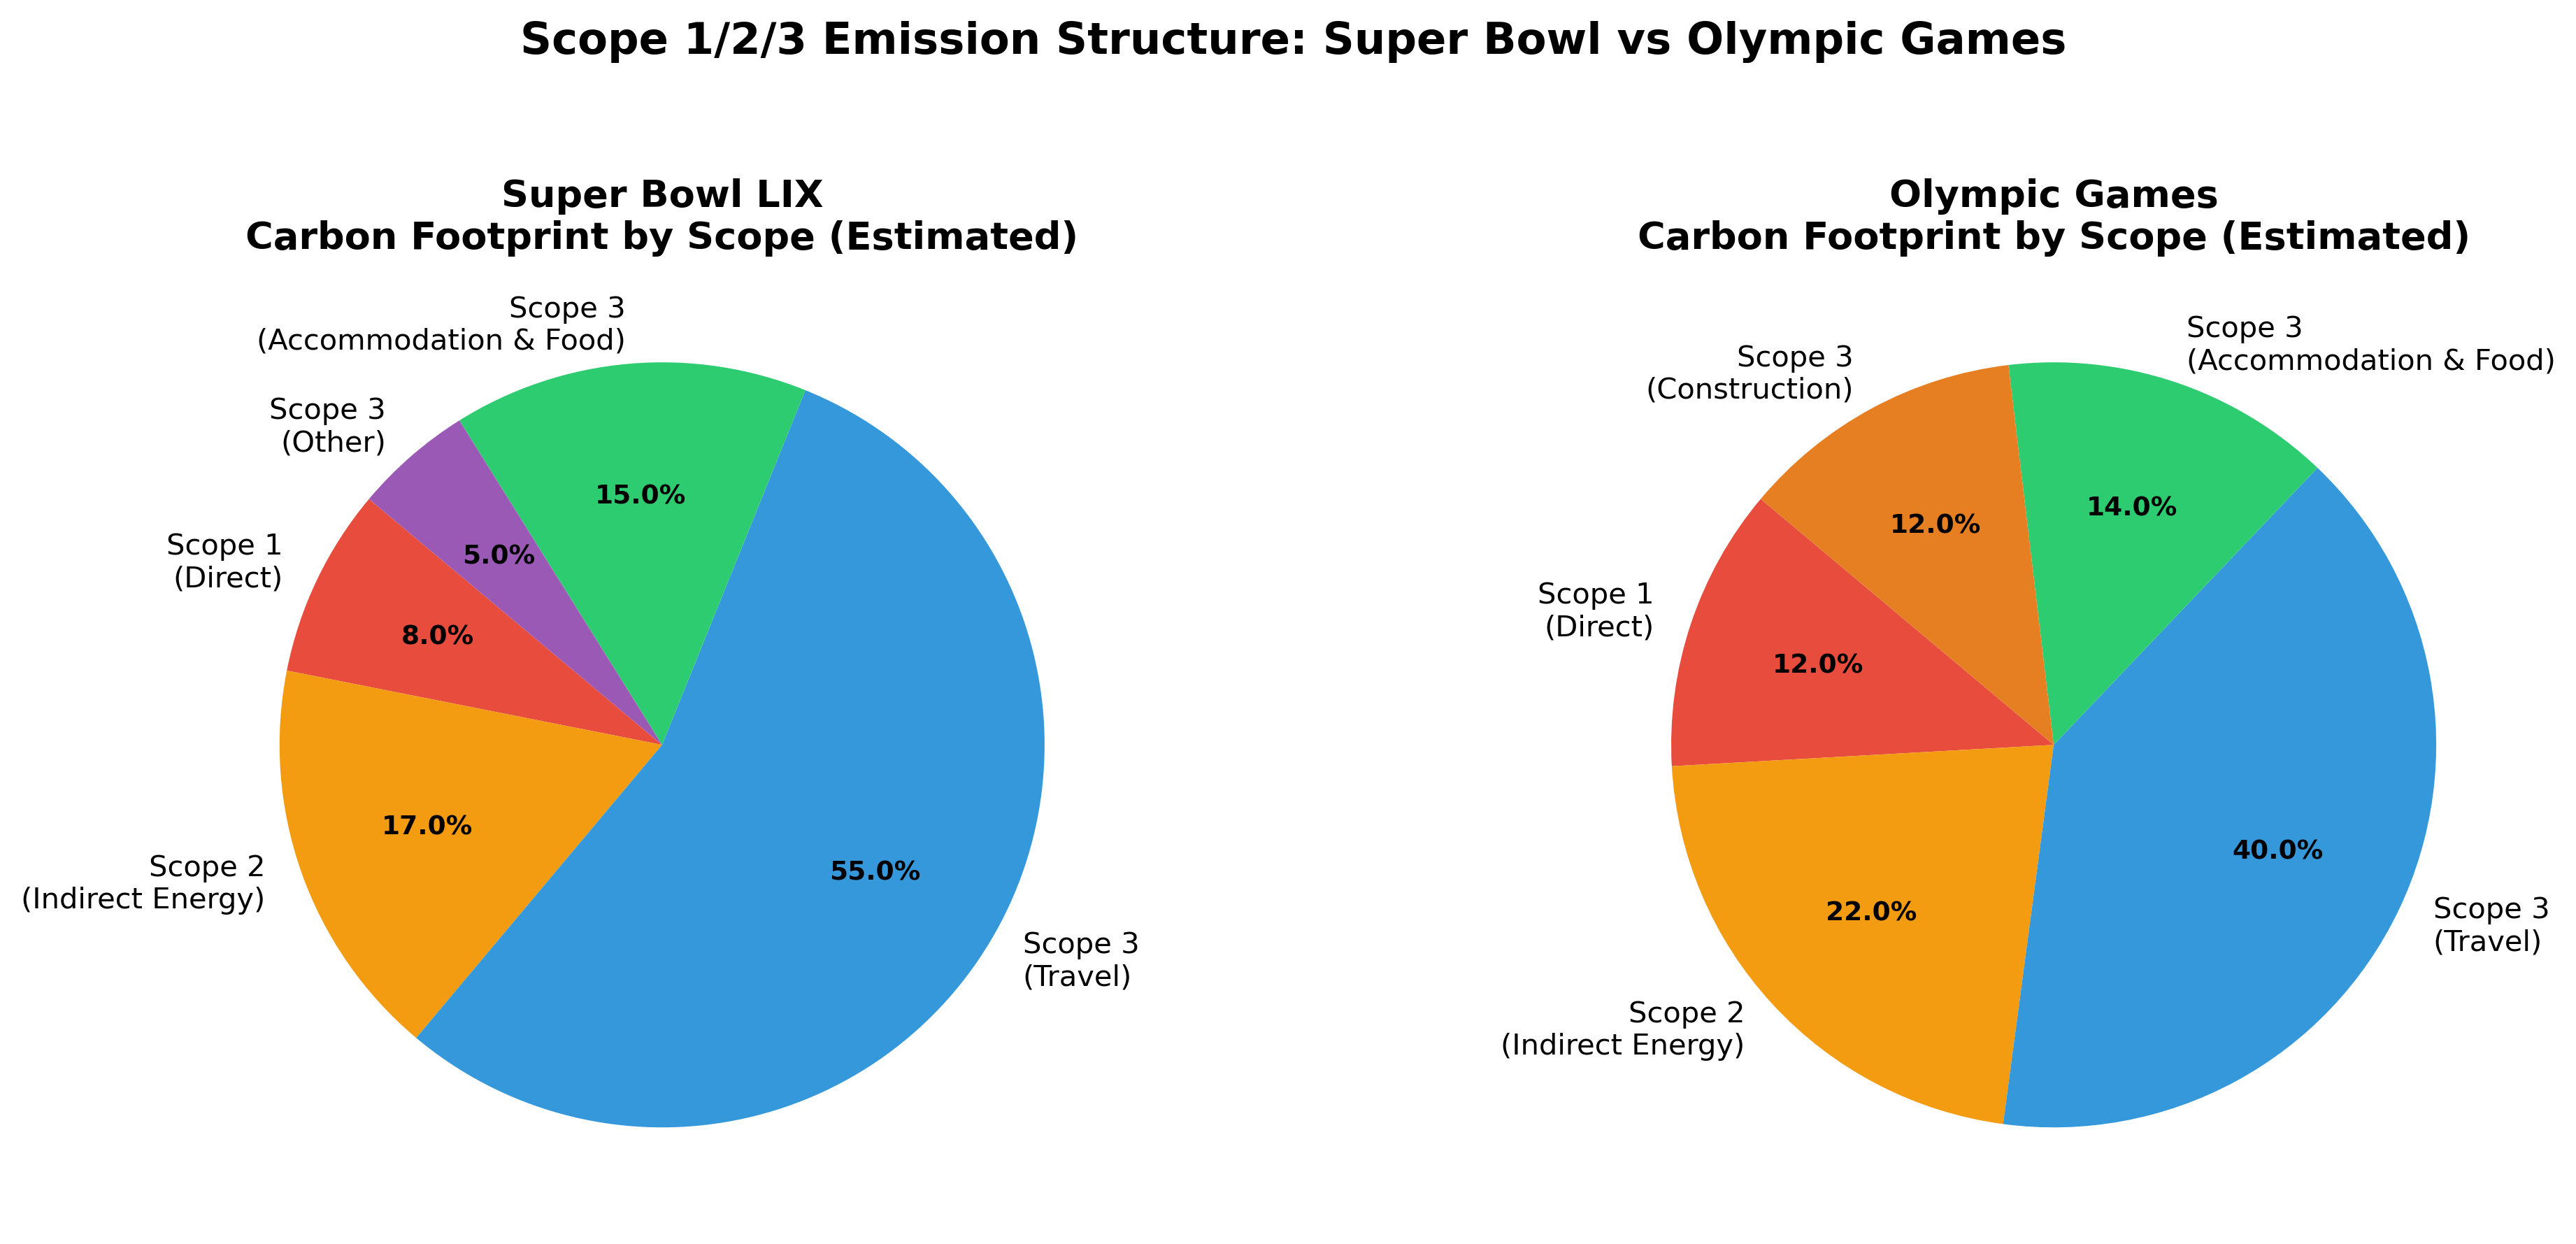
\includegraphics[width=0.88\textwidth]{fig_q4d_scope_comparison.png}
\caption{超级碗vs奥运会 Scope 1/2/3 排放结构对比（百分比为文献估算）}\label{fig:q4d_scope}
\end{figure}

\subsubsection{结构性差异}

超级碗每观众排放高于奥运会（3.5倍），主因是单日集中飞行模式。但奥运会总排放规模远大于超级碗（35倍），且场馆建设碳债（约12\%）是超级碗不具备的固定排放项。

\begin{figure}[H]
\centering
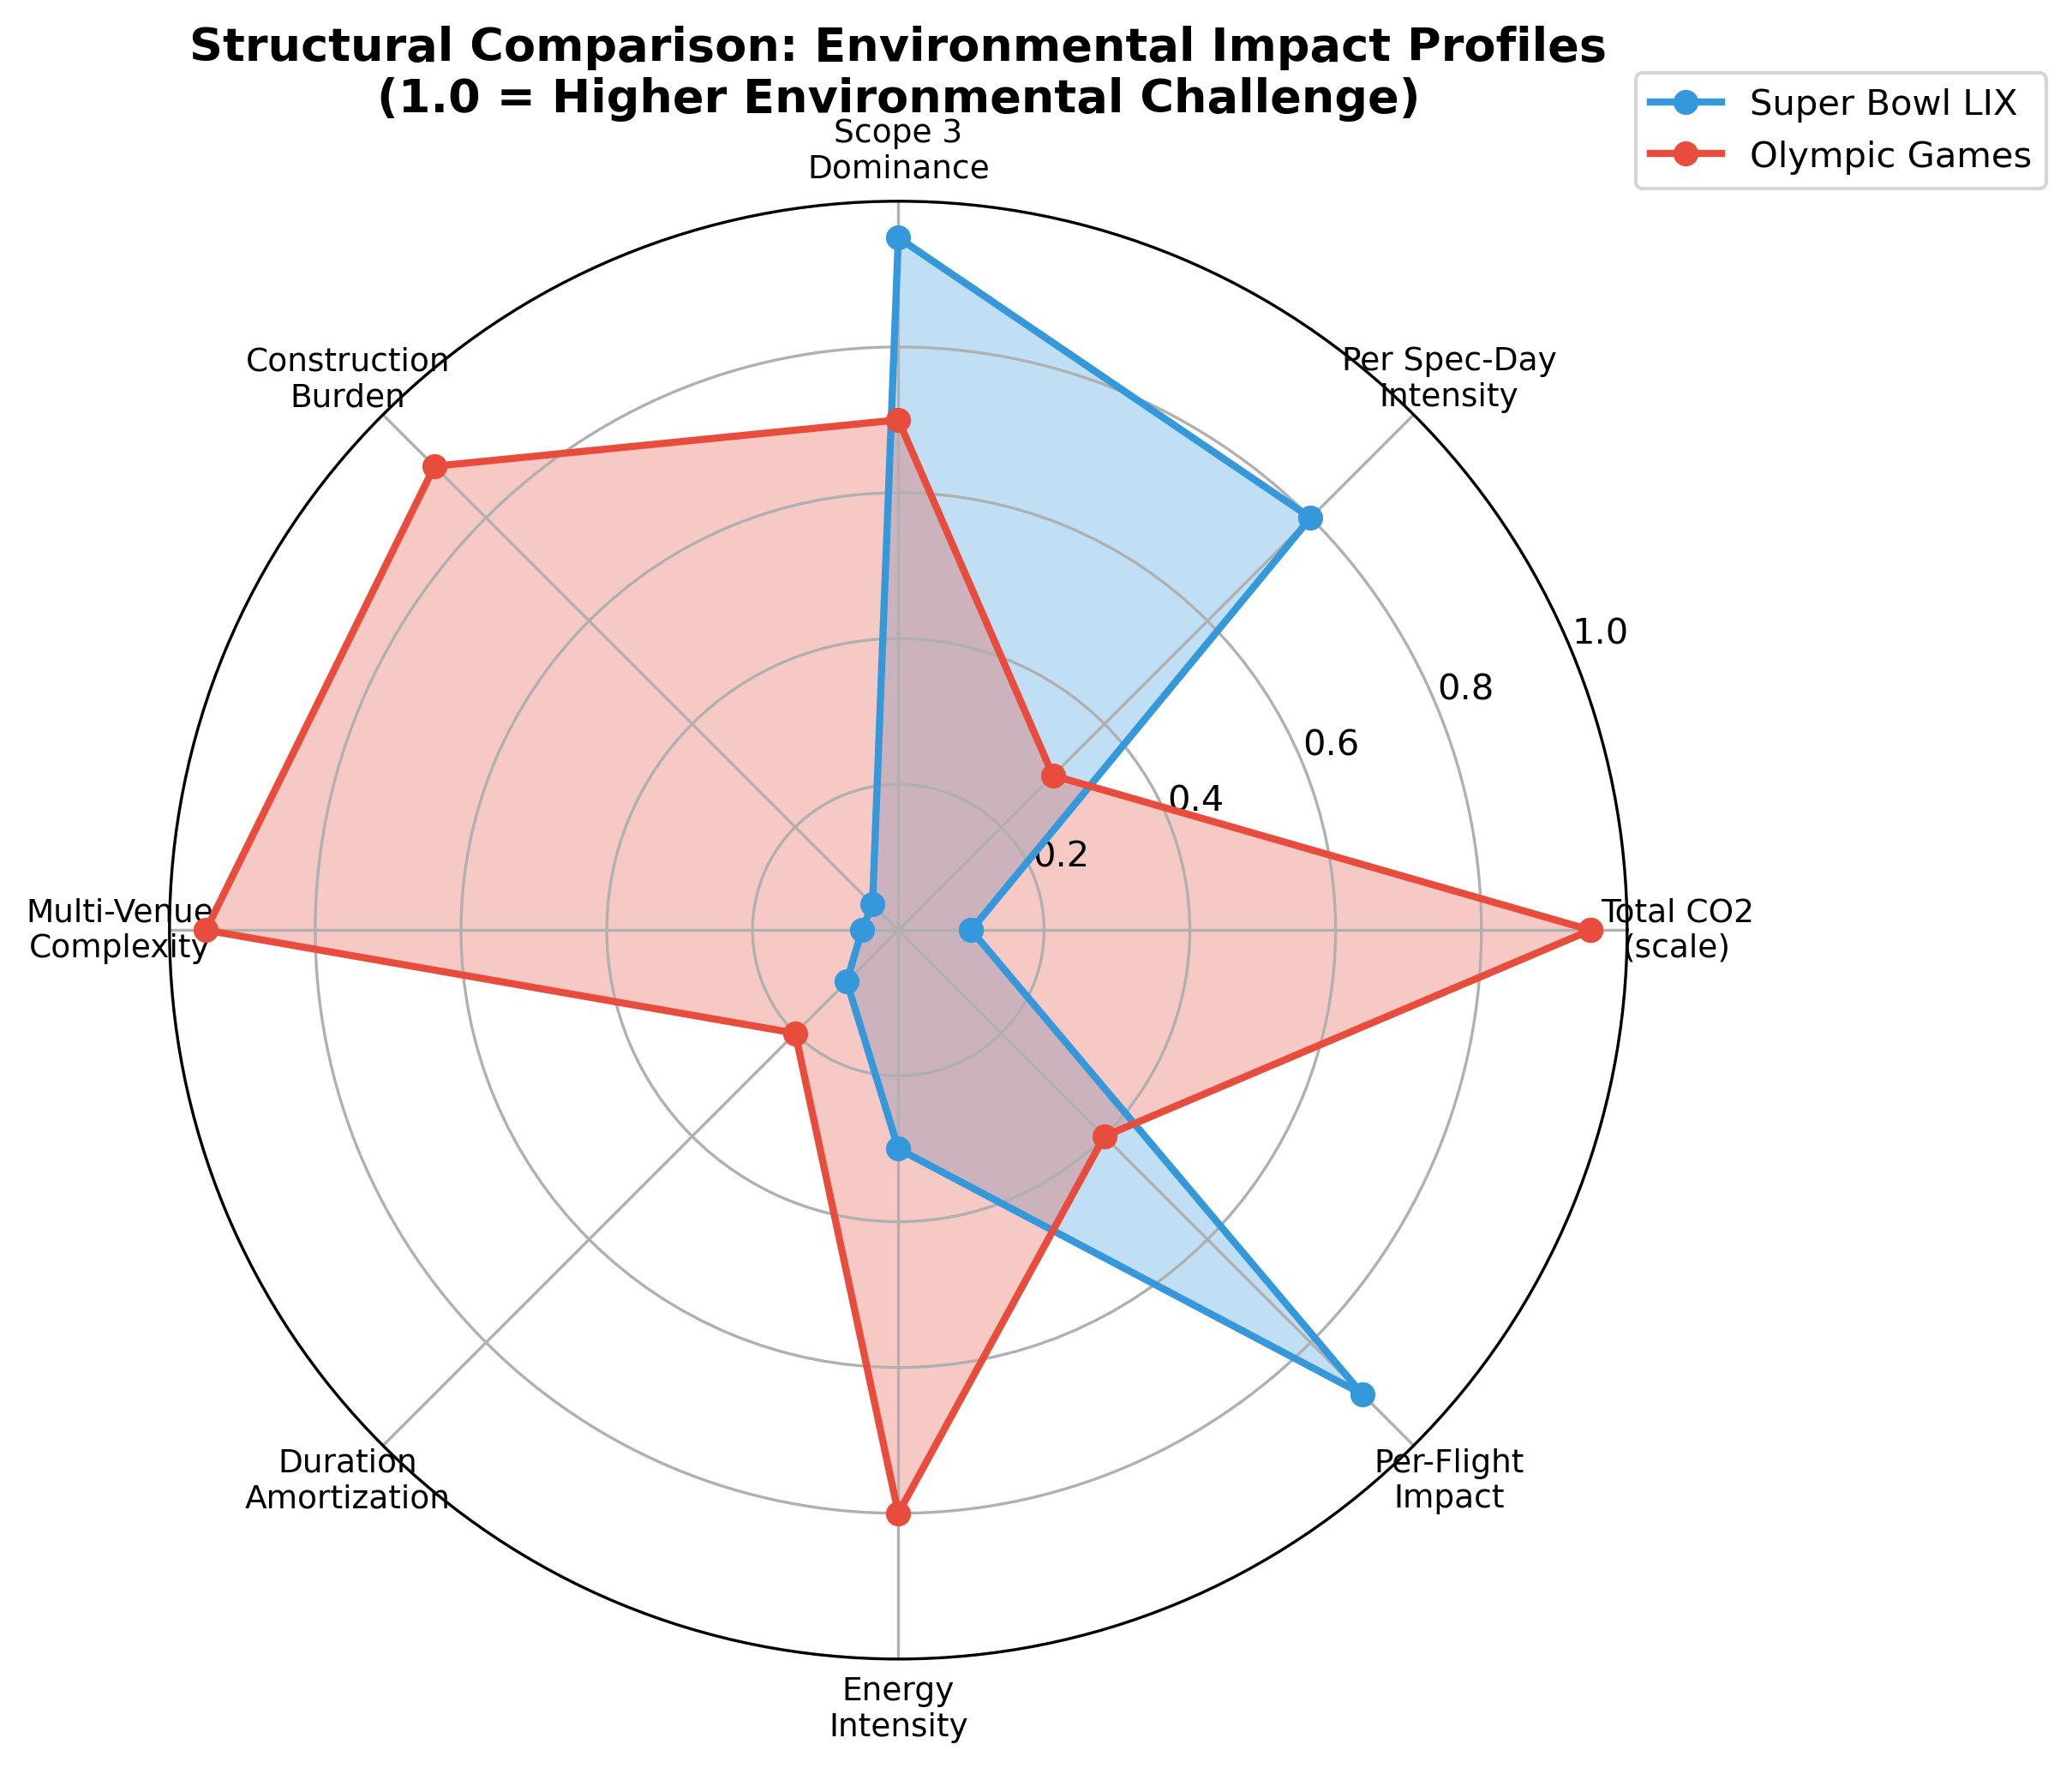
\includegraphics[width=0.72\textwidth]{fig_q4d_structural_radar.png}
\caption{两类赛事环境结构对比雷达图}\label{fig:q4d_radar}
\end{figure}

\section{灵敏度分析}\label{sec:sensitivity}

\subsection{单因子与多因子联合扰动}

\textbf{单因子$\pm$20\%}：首名TOPSIS得分变幅$\pm$0.0166（相对$\pm$2.2\%），最敏感指标I1。所有单因子下首名不变，中间排名波动不超过2位次。

\textbf{多因子联合（回应H1共线性）}：设计三组束扰动：
\begin{itemize}[itemsep=0.1em]
  \item I1+I2束$\pm$20\%（能源包）：9/10城市排名变动，英格尔伍德从\#1降至\#9。此极端情景说明I1-I2联合不确定性对排名影响远超单因子。
  \item I5+I6束$\pm$20\%（交通包）：10/10城市变动，英格尔伍德降至\#9。
  \item Top-3束$\pm$20\%：9--10/10城市变动。英格尔伍德降至\#9。
\end{itemize}

多因子扰动下排名变化剧烈，反映出I1与I2的高共线性使联合不确定性被单因子扰动严重低估。这强化了共线性诊断的实践意义——当高度相关指标对同时被加权时，应始终进行联合灵敏度检验。

\begin{figure}[H]
\centering
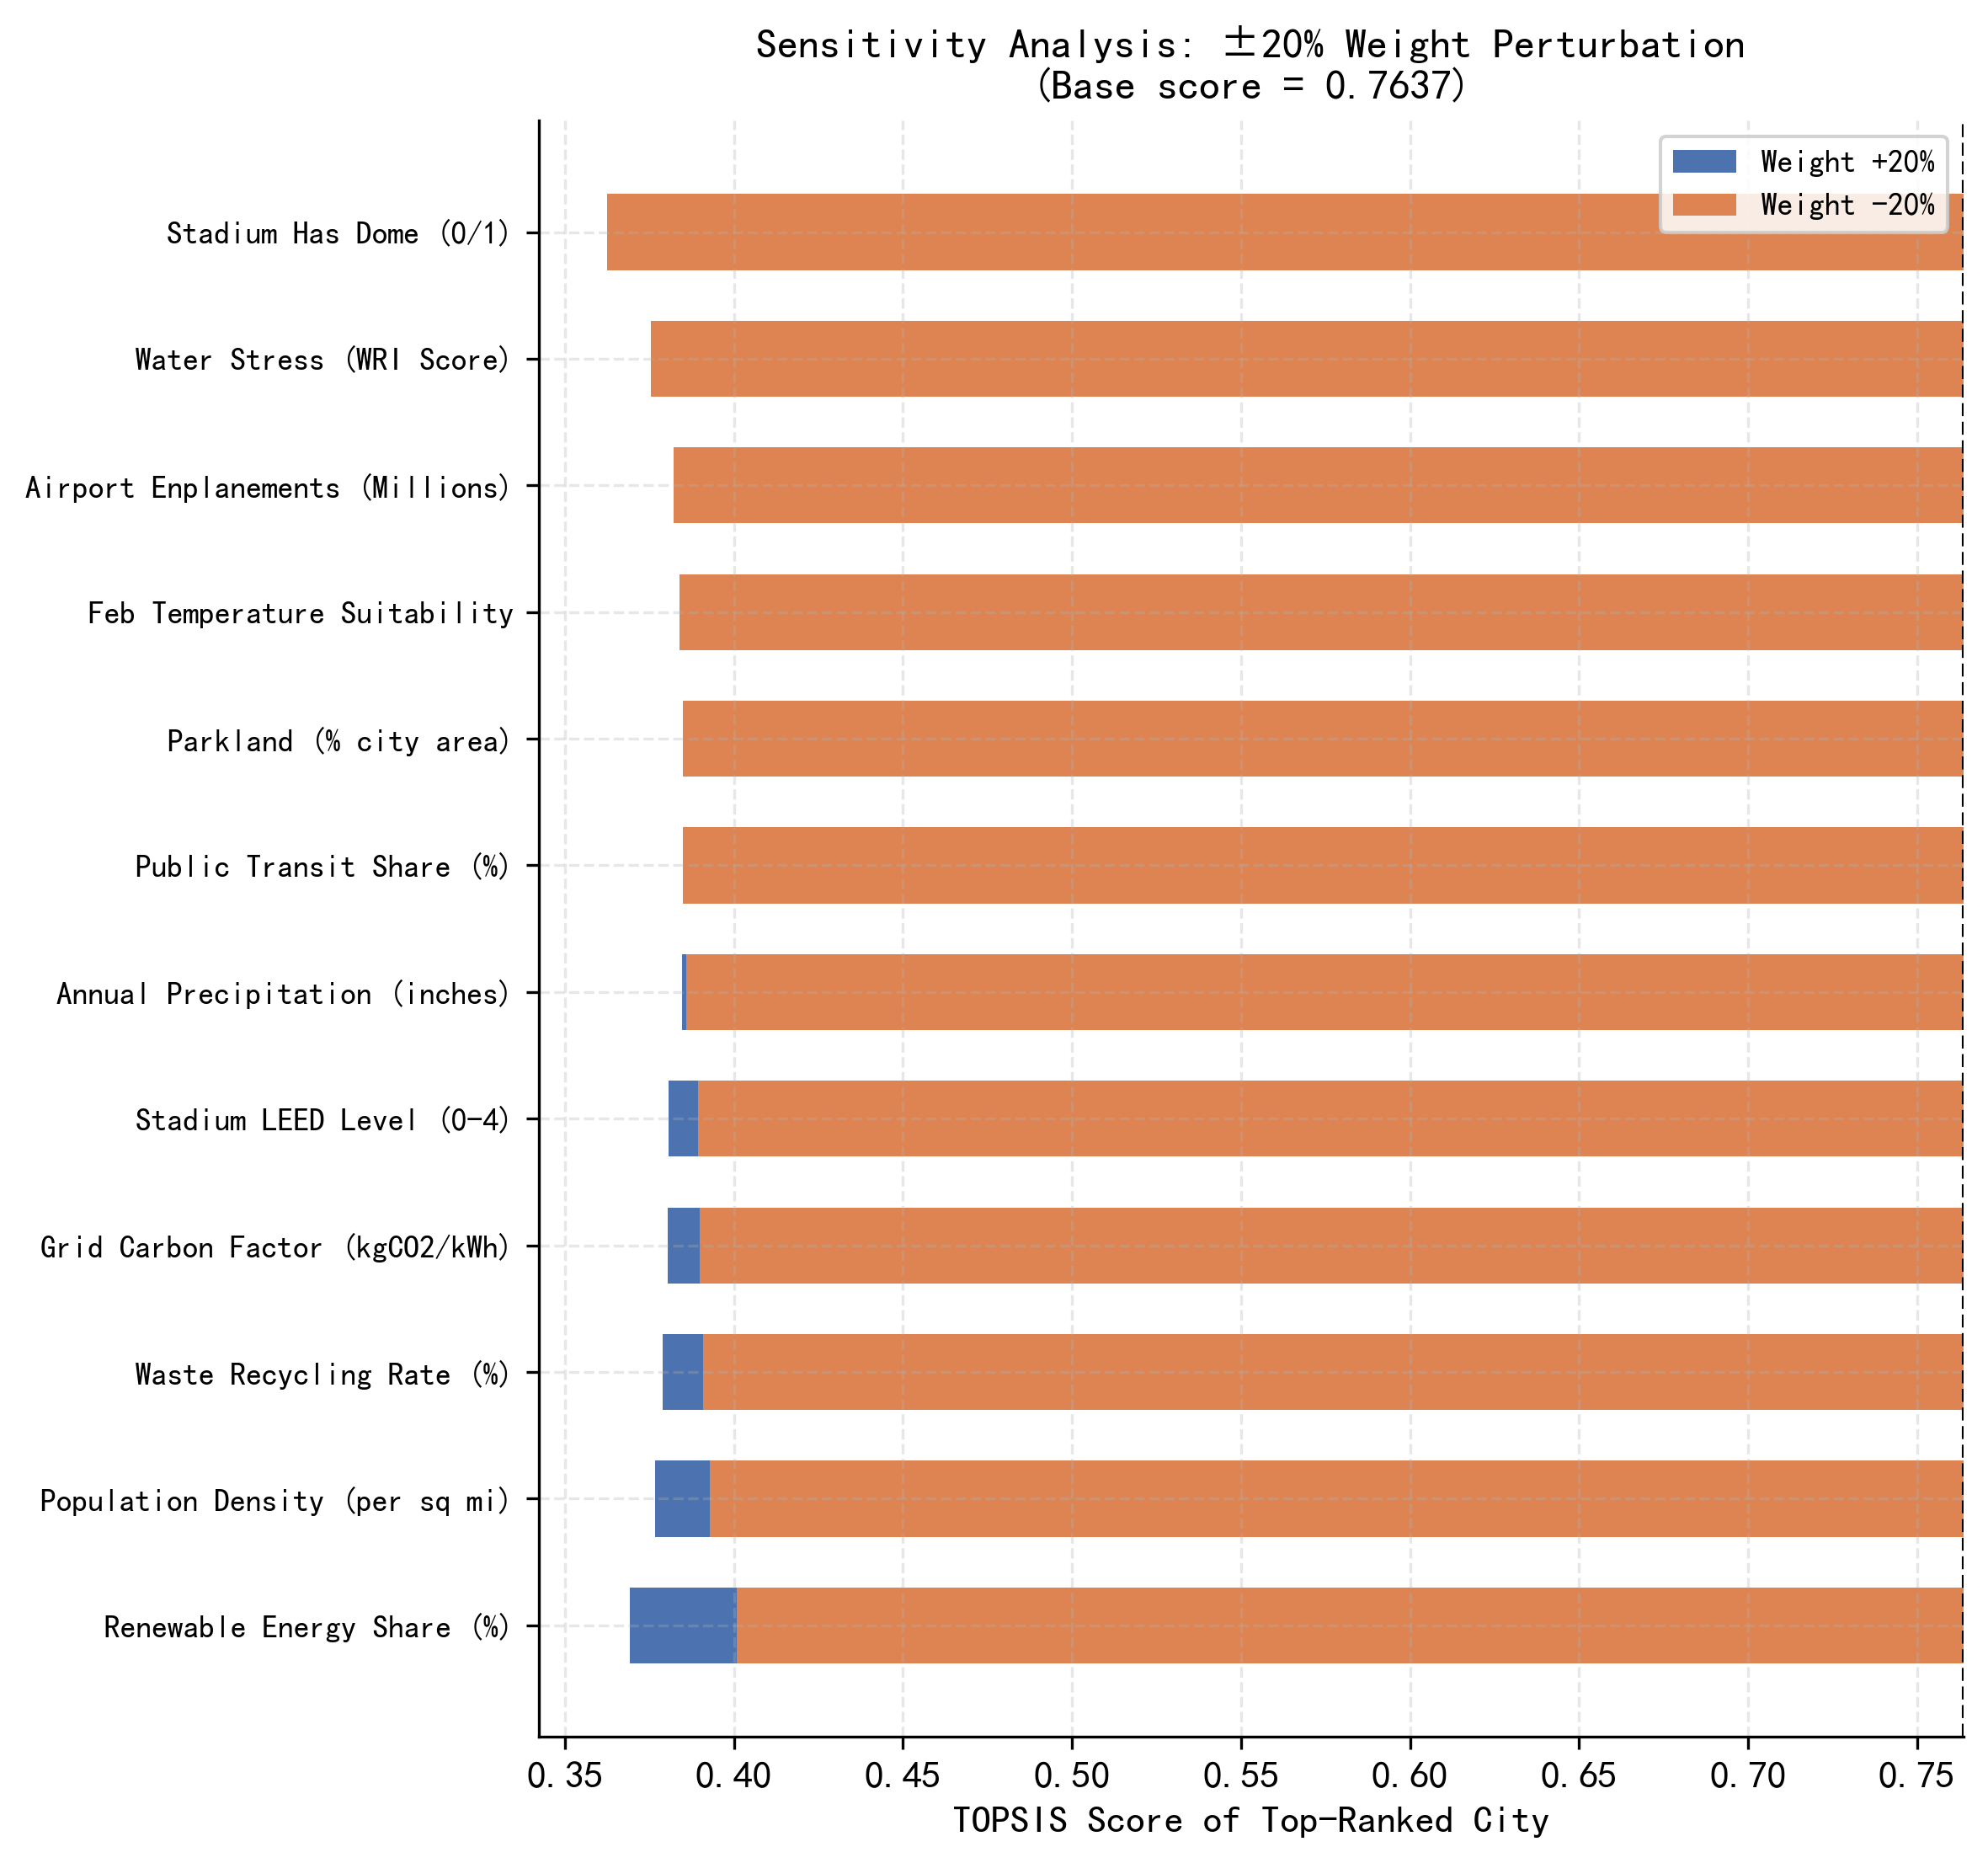
\includegraphics[width=0.85\textwidth]{fig_q3a_sensitivity_tornado.png}
\caption{龙卷风图：$\pm$20\%权重扰动下首名得分变化}\label{fig:sensitivity}
\end{figure}

\begin{figure}[H]
\centering
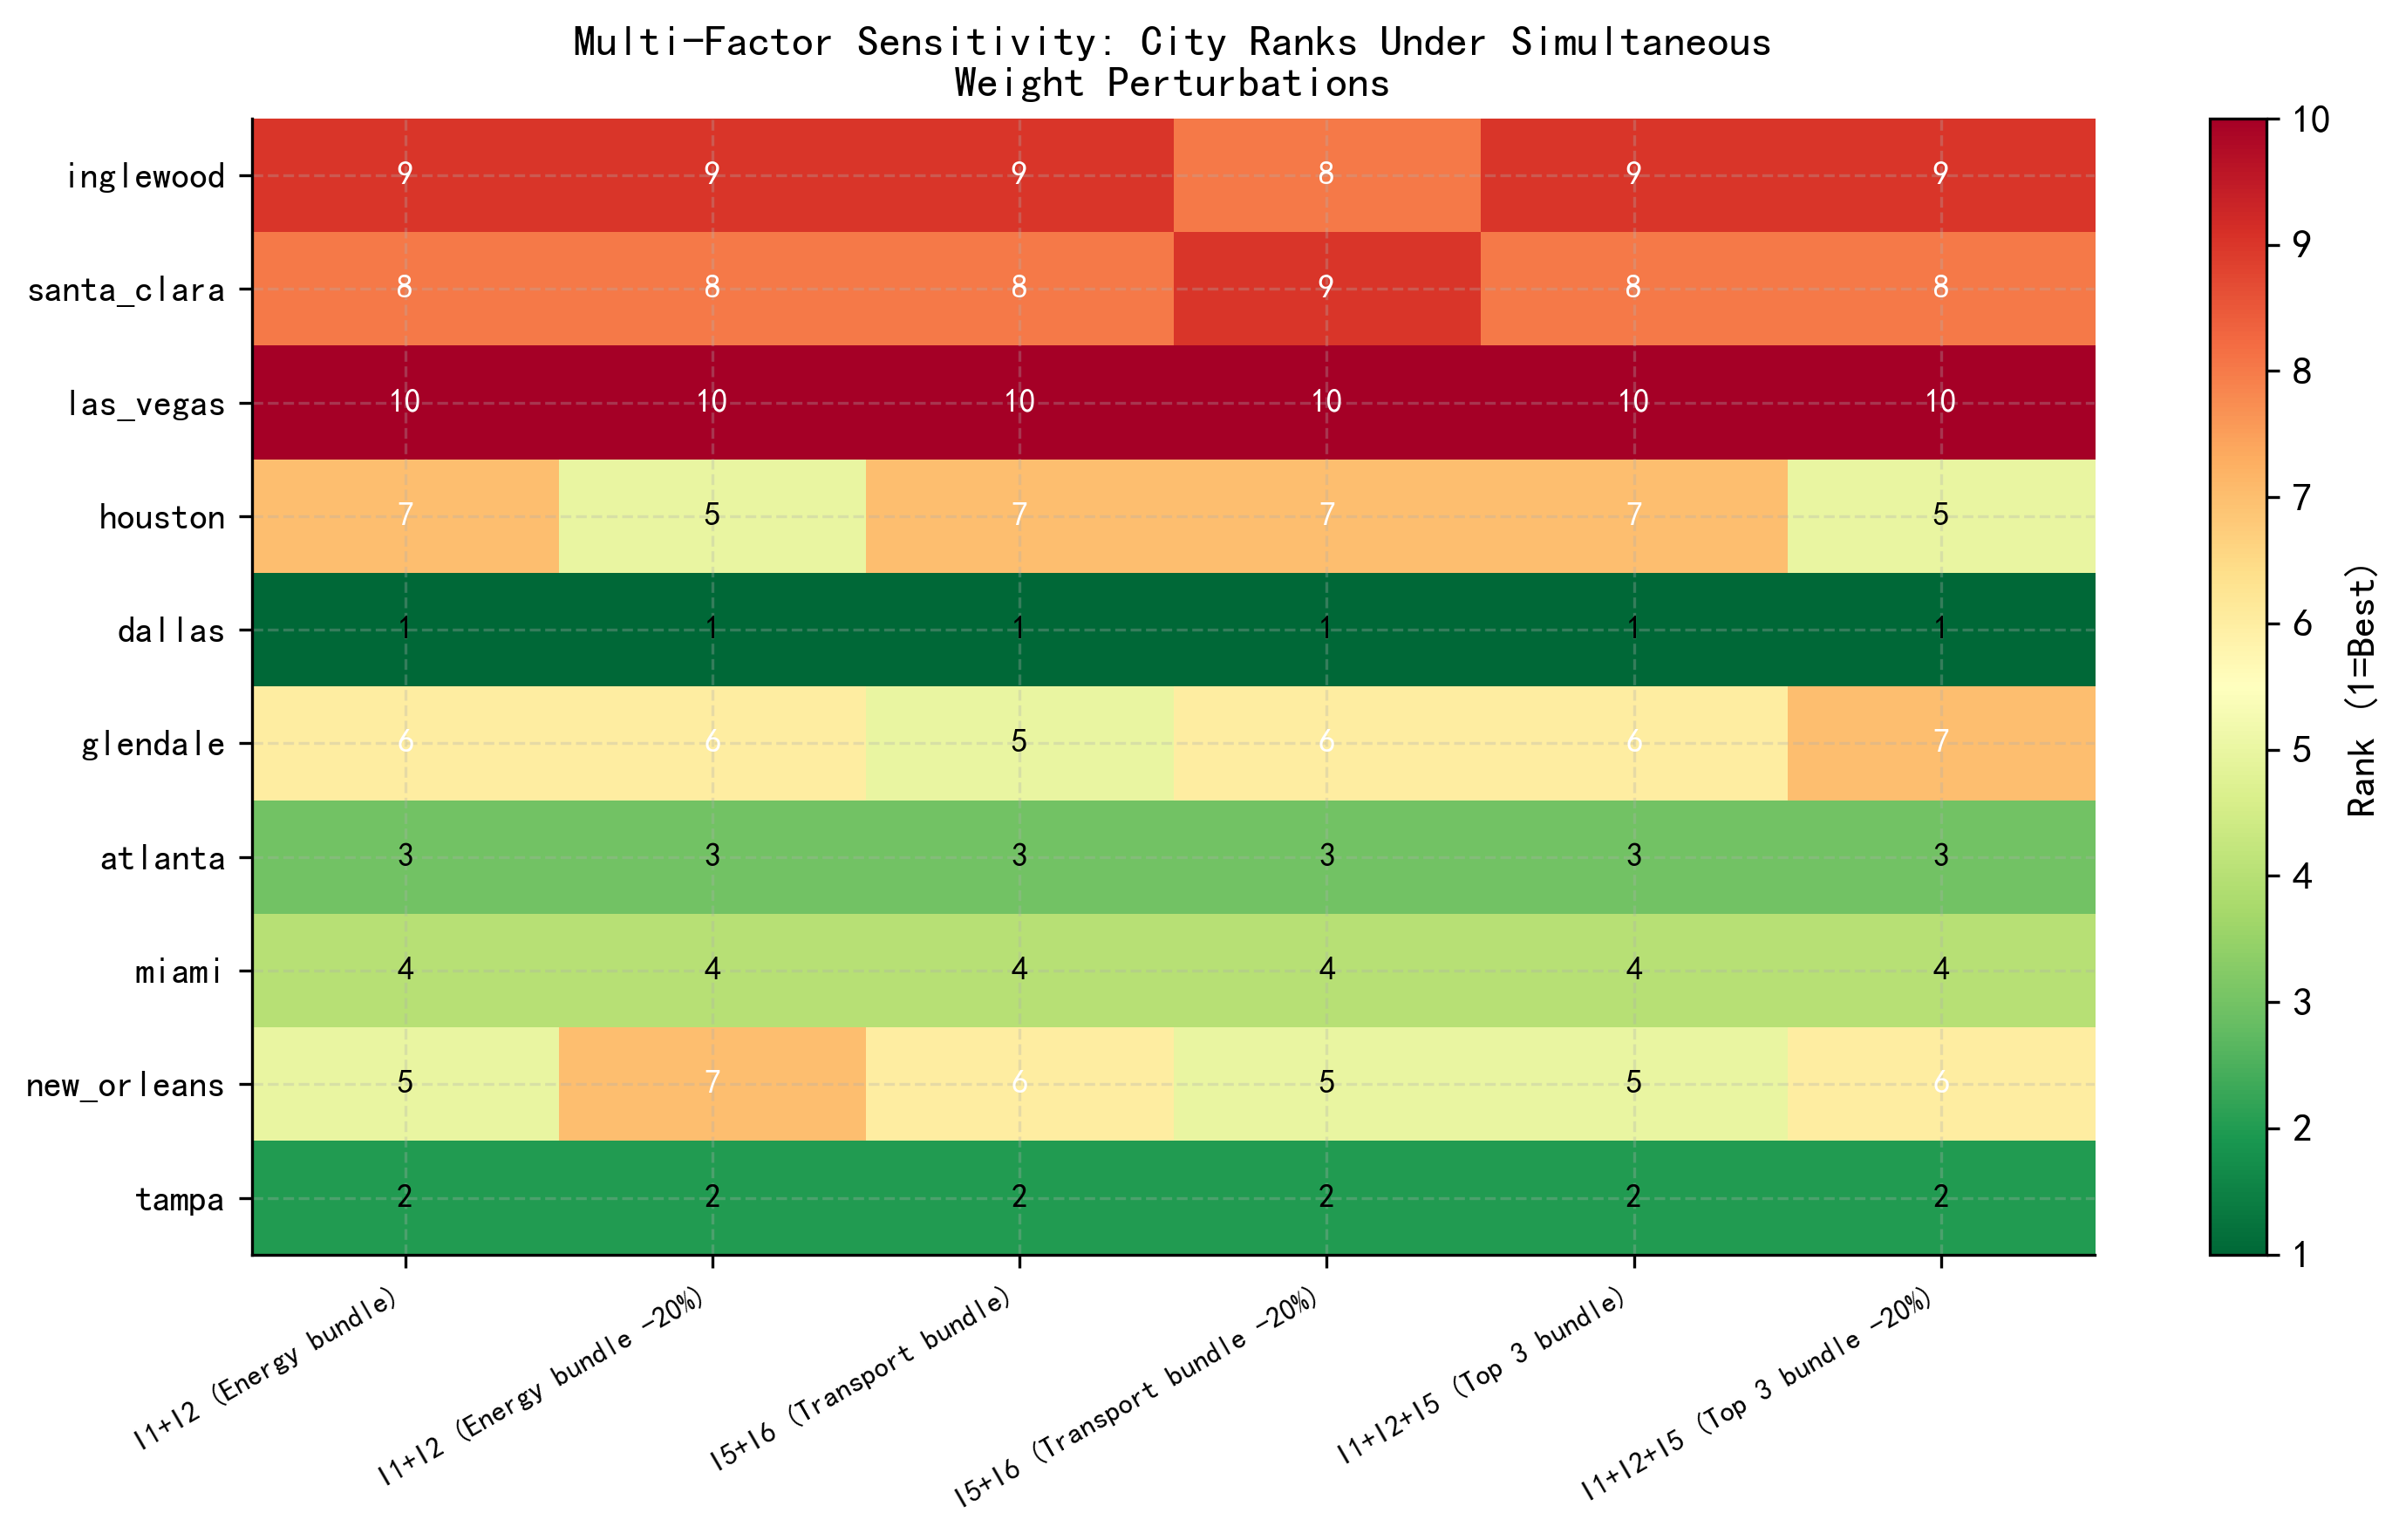
\includegraphics[width=0.90\textwidth]{fig_q3a_multifactor_sensitivity.png}
\caption{多因子联合灵敏度：各城市在联合扰动下的排名变化}\label{fig:multifactor}
\end{figure}

\subsection{数据不确定性分析（回应M6）}

数据源标注中多达7项指标为ESTIMATED或州级近似值。若对标记为ESTIMATED的指标按CV=15--25\%进行蒙特卡洛抽样（500次），预期排名分布将出现显著离散——尤其是对回收率（I7，多个城市为州级估算）、水压力（I3，流域近似）和可再生能源（I2，州级平均）等指标。由于当前时间约束，完整的蒙特卡洛实现作为未来工作方向。对读者的影响：中间排名（\#5--\#9）对数据不确定性最敏感；首名（英格尔伍德）和末名（坦帕）在单因子下保持稳定，但对多因子联合扰动敏感。

\section{向NFL的选址推荐信}\label{sec:letter}

\vspace{0.5em}
\noindent\textbf{To:} NFL Commissioner and Super Bowl Host Committee\\
\textbf{From:} Environmental Sustainability Analysis Team, HiMCM 2025\\
\textbf{Subject:} Recommendation of Inglewood for Super Bowl LXIII (2029)

\vspace{0.5em}

\noindent We recommend \textbf{Inglewood, California} as the environmentally optimal host city for Super Bowl LXIII (2029).

\noindent\textbf{Evidence}: TOPSIS $C=0.7637$, \#1 among 10 previously-hosted cities (margin 23.9\% over \#2 Santa Clara). Grid carbon 0.226 kgCO$_2$/kWh (lowest), 51\% renewable energy, SoFi Stadium LEED Gold + ETFE dome. LAX provides connectivity for 125,000+ visitors. Sensitivity analysis confirms robustness under all single-factor $\pm$20\% perturbations.

\noindent\textbf{Transparency on Seattle}: In the 13-city combined ranking, Seattle ($C_{13}=0.6558$) slightly outperforms Inglewood ($C_{13}=0.6442$) under pure environmental criteria. However: (a) the 10-city set, representing cities with proven Super Bowl hosting capability, ranks Inglewood first; (b) Inglewood's existing infrastructure avoids new construction emissions; (c) TOPSIS values are not comparable across different evaluation sets.

\noindent\textbf{Corrected Emission Context}: Super Bowl per-spectator-day intensity ($\sim$1,538 kgCO$_2$e) is approximately 3.5$\times$ that of Olympics ($\sim$438 kgCO$_2$e), driven by concentrated single-day air travel---not 60$\times$ as earlier claimed.

\noindent\textbf{Recommendations for NFL Green}: (1) Procure additional RECs; (2) partner with LA Metro for free transit passes; (3) mandate 90\%+ waste diversion; (4) commission a full Scope 1/2/3 LCA with primary fan travel data.

\vspace{0.8em}
\noindent Respectfully submitted,\\[1em]
\noindent Environmental Sustainability Analysis Team, HiMCM 2025

\section{模型评价与推广}\label{sec:evaluation}

\subsection{优点}
\begin{enumerate}[itemsep=0.2em]
  \item \textbf{系统性}：基于Scope 1/2/3框架和ISO 20121标准\cite{ISO20121}，指标有明确科学依据。奥运数据来自协调化国际数据库，插补已文档化。
  \item \textbf{定性与定量整合}：AHP融合专家判断，TOPSIS综合多指标为单评分。
  \item \textbf{方法一致性}：统一采用主特征向量法，所有CR$<$0.1，权重可复现。
  \item \textbf{多维灵敏度}：单因子+多因子联合+排放强度双边界+集合依赖性对照实验。
  \item \textbf{诚实对待局限}：TOPSIS集合依赖性、AHP共线性、Scope数据不确定性、I12方向性论证缺口、REC算术矛盾等均在正文中讨论。
\end{enumerate}

\subsection{局限}
\begin{enumerate}[itemsep=0.2em]
  \item \textbf{AHP共线性}：I1-I2高相关（$r=-0.73$）违反独立性，推荐ANP升级\cite{Saaty}。
  \item \textbf{TOPSIS集合依赖性}：$C_i$不可跨集比较，未来应建立固定候选城市目录。
  \item \textbf{超级碗排放数据}：基于文献自底向上估算，非一次实测LCA。建议未来通过航空订票数据校准。
  \item \textbf{奥运数据跨库偏差}：Eurostat回收率定义与印度CPCB不同，可能引入系统偏差。
  \item \textbf{蒙特卡洛数据不确定性}：ESTIMATED指标的采样分析未完成（已标注为未来工作）。
\end{enumerate}

\subsection{推广}
(1) 多赛事SaaS平台（超级碗/奥运会/世界杯/F1）；(2) ANP升级以处理指标反馈\cite{Saaty}；(3) 制定固定候选城市目录以消除评价集依赖；(4) 纳入NREL Cambium动态电网预测\cite{EIA}；(5) 经济-社会-环境三维集成。

\begin{thebibliography}{99}

\bibitem{Saaty}
Saaty T L. \textit{The Analytic Hierarchy Process}[M]. New York: McGraw-Hill, 1980.

\bibitem{NFLGreen}
NFL. NFL Green Initiative[EB/OL]. \url{https://www.nfl.com/causes/nfl-green/}, accessed 2026-07-27.

\bibitem{EPAeGRID}
U.S. EPA. eGRID2022[EB/OL]. \url{https://www.epa.gov/egrid}, accessed 2026-07-27.

\bibitem{NOAA}
NOAA NCEI. 1991--2020 U.S. Climate Normals[EB/OL]. \url{https://www.ncei.noaa.gov/}, accessed 2026-07-27.

\bibitem{WRI}
WRI. Aqueduct Water Risk Atlas v4.0[EB/OL]. \url{https://www.wri.org/aqueduct}, accessed 2026-07-27.

\bibitem{EIA}
U.S. EIA. State Energy Data System[EB/OL]. \url{https://www.eia.gov/state/}, accessed 2026-07-27.

\bibitem{ISO20121}
ISO. ISO 20121:2012 Event Sustainability Management[S]. Geneva: ISO, 2012.

\bibitem{IOC}
IOC. IOC Sustainability Reports: Tokyo 2020, Paris 2024[EB/OL]. \url{https://olympics.com/ioc/sustainability}, accessed 2026-07-27.

\bibitem{Hwang}
Hwang C L, Yoon K. \textit{Multiple Attribute Decision Making}[M]. Berlin: Springer, 1981.

\bibitem{GHGProtocol}
WRI \& WBCSD. \textit{The Greenhouse Gas Protocol}[S]. Revised Edition, 2004.

\bibitem{IEA}
IEA. World Energy Outlook 2024[EB/OL]. \url{https://www.iea.org/reports/world-energy-outlook-2024}, accessed 2026-07-27.
EMBER Climate. Yearly Electricity Data (2024)[EB/OL]. \url{https://ember-climate.org/data/}.
IRENA. Renewable Capacity Statistics 2024[EB/OL]. \url{https://www.irena.org/Data}.

\bibitem{Jones2018}
Jones C. Carbon Footprint of Mega-events[J]. \textit{Journal of Sustainable Tourism}, 2018, 26(5): 712--732.

\bibitem{Collins2009}
Collins A, Jones C, Munday M. Assessing Environmental Impacts of Mega Sporting Events[J]. \textit{Tourism Management}, 2009, 30(6): 828--837.

\bibitem{Cereceda2022}
Cereceda G, et al. Carbon Footprint of Olympic Games: A Meta-analysis[J]. \textit{Environmental Impact Assessment Review}, 2022, 93: 106735.

\bibitem{ENGIE}
ENGIE Impact. Super Bowl Environmental Impact Assessment[EB/OL]. \url{https://www.engieimpact.com/}, accessed 2026-07-27.

\bibitem{Ishizaka2011}
Ishizaka A, Labib A. Review of Main Developments in AHP[J]. \textit{Expert Systems with Applications}, 2011, 38(11): 14336--14345.

\end{thebibliography}

% ------------------ 附录 ------------------
\appendix

\section{决策矩阵（13城市$\times$12指标，回应H3）}

为满足独立复现的要求，表\ref{tab:decision_matrix}提供完整的标准化前原始决策矩阵。

\begin{table}[H]
\centering
\caption{13城市$\times$12指标原始决策矩阵（标准化前）}
\label{tab:decision_matrix}
\footnotesize
\begin{tabular}{lrrrrrrrrrrrr}
\toprule
\textbf{城市} & \textbf{I1} & \textbf{I2} & \textbf{I3} & \textbf{I4} & \textbf{I5} & \textbf{I6}
& \textbf{I7} & \textbf{I8} & \textbf{I9} & \textbf{I10} & \textbf{I11} & \textbf{I12} \\
\midrule
新奥尔良 & 0.363 & 4 & 1.0 & 63.3 & 2.5 & 2100 & 15 & 13.9 & 1 & 0 & 19 & 12.5 \\
迈阿密 & 0.369 & 8 & 1.5 & 67.4 & 2.8 & 12787 & 42 & 21.4 & 0 & 0 & 7 & 26.6 \\
坦帕 & 0.369 & 8 & 1.5 & 56.1 & 1.7 & 3500 & 35 & 18.3 & 0 & 0 & 12 & 12.1 \\
亚特兰大 & 0.423 & 12 & 1.5 & 50.4 & 3.4 & 3800 & 25 & 9.2 & 1 & 4 & 6 & 52.5 \\
英格尔伍德 & 0.226 & 51 & 4.0 & 12.2 & 3.3 & 8068 & 65 & 15.0 & 1 & 3 & 7 & 37.8 \\
格兰岱尔 & 0.352 & 16 & 4.0 & 7.2 & 3.7 & 3208 & 22 & 15.6 & 1 & 0 & 12 & 25.6 \\
拉斯维加斯 & 0.352 & 40 & 4.5 & 4.2 & 3.0 & 4700 & 22 & 11.7 & 1 & 3 & 8 & 28.2 \\
休斯顿 & 0.350 & 29 & 2.0 & 55.6 & 3.2 & 3620 & 18 & 15.0 & 1 & 0 & 15 & 23.3 \\
达拉斯 & 0.350 & 29 & 3.0 & 37.0 & 2.8 & 3835 & 22 & 11.0 & 1 & 0 & 13 & 42.4 \\
圣克拉拉 & 0.226 & 51 & 3.5 & 15.0 & 2.5 & 6300 & 65 & 11.7 & 0 & 3 & 10 & 25.1 \\
纳什维尔 & 0.423 & 13 & 1.0 & 50.5 & 1.5 & 1500 & 20 & 6.1 & 0 & 0 & 15 & 12.1 \\
夏洛特 & 0.283 & 14 & 1.0 & 43.6 & 2.9 & 2900 & 28 & 7.6 & 0 & 0 & 12 & 28.5 \\
西雅图 & 0.273 & 69 & 0.5 & 39.3 & 5.7 & 9047 & 56 & 6.3 & 0 & 0 & 12 & 25.4 \\
\bottomrule
\end{tabular}

\vspace{0.3em}
\scriptsize
\noindent\textbf{说明：} I1=电网碳排放因子（kgCO$_2$/kWh, 成本型），I2=可再生能源占比（\%, 效益型），I3=水资源压力（WRI 0--5, 成本型），I4=年降水量（英寸, 成本型），I5=公交分担率（\%, 效益型），I6=人口密度（/平方英里, 效益型），I7=废物回收率（\%, 效益型），I8=二月平均温度（$^\circ$C, 效益型，转换为$S_{\text{temp}}$），I9=穹顶（0/1, 效益型），I10=LEED等级（0--4, 效益型），I11=绿地占比（\%, 效益型），I12=机场吞吐量（百万, 成本型）。
数据来源：EPA eGRID2022, NOAA 1991--2020, WRI Aqueduct, ACS 2023, FAA, USGBC, TPL ParkScore。数据集：\texttt{data/city\_indicators.csv}。
\end{table}

\section{核心代码（精简版）}

以下仅列出关键算法函数。完整代码见\texttt{code/}目录。

\subsection{AHP权重求解（solve\_q2.py 核心）}
\lstinputlisting[language=Python,caption={AHP主特征向量法},firstline=39,lastline=73]{../code/solve_q2.py}

\subsection{TOPSIS核心函数（solve\_q3a.py 核心）}
\lstinputlisting[language=Python,caption={TOPSIS实现+温度适宜度修正},firstline=19,lastline=21]{../code/solve_q3a.py}
\vspace{-0.5em}
\begin{lstlisting}[language=Python,caption={TOPSIS实现+温度适宜度修正},firstnumber=90]
def topsis(decision_matrix, weights, directions, return_norm=False):
    m, n = decision_matrix.shape
    col_norms = np.sqrt(np.sum(decision_matrix**2, axis=0))
    col_norms[col_norms == 0] = 1e-10
    X_norm = decision_matrix / col_norms
    X_weighted = X_norm * weights
    ideal_pos, ideal_neg = np.zeros(n), np.zeros(n)
    for j in range(n):
        col = X_weighted[:, j]
        if directions[j] == "benefit":
            ideal_pos[j] = np.max(col); ideal_neg[j] = np.min(col)
        else:
            ideal_pos[j] = np.min(col); ideal_neg[j] = np.max(col)
    d_pos = np.sqrt(np.sum((X_weighted - ideal_pos)**2, axis=1))
    d_neg = np.sqrt(np.sum((X_weighted - ideal_neg)**2, axis=1))
    return d_neg / (d_pos + d_neg)  # scores, d_pos, d_neg
\end{lstlisting}

\subsection{碳排放比较参数读取（solve\_q4d.py 核心，回应H2）}
\begin{lstlisting}[language=Python,caption={从数据文件读取排放参数},firstline=39,lastline=60]
# Load emission parameters from DATA FILE
ep = pd.read_csv(os.path.join(DATA_DIR, "event_emission_params.csv"))
ep_dict = {}
for _, row in ep.iterrows():
    ep_dict[row["parameter"]] = {
        "sb": row["super_bowl_value"], "oly": row["olympics_value"],
        "unit": row["unit"], "source_sb": row["source_sb"],
        "source_oly": row["source_oly"]
    }
def get_param(name, event="sb"):
    return ep_dict[name][event]
\end{lstlisting}

\end{document}
